% Options for packages loaded elsewhere
\PassOptionsToPackage{unicode}{hyperref}
\PassOptionsToPackage{hyphens}{url}
\PassOptionsToPackage{dvipsnames,svgnames,x11names}{xcolor}
%
\documentclass[
  12pt,
  letterpaper,
]{book}

\usepackage{amsmath,amssymb}
\usepackage{iftex}
\ifPDFTeX
  \usepackage[T1]{fontenc}
  \usepackage[utf8]{inputenc}
  \usepackage{textcomp} % provide euro and other symbols
\else % if luatex or xetex
  \usepackage{unicode-math}
  \defaultfontfeatures{Scale=MatchLowercase}
  \defaultfontfeatures[\rmfamily]{Ligatures=TeX,Scale=1}
\fi
\usepackage{lmodern}
\ifPDFTeX\else  
    % xetex/luatex font selection
\fi
% Use upquote if available, for straight quotes in verbatim environments
\IfFileExists{upquote.sty}{\usepackage{upquote}}{}
\IfFileExists{microtype.sty}{% use microtype if available
  \usepackage[]{microtype}
  \UseMicrotypeSet[protrusion]{basicmath} % disable protrusion for tt fonts
}{}
\makeatletter
\@ifundefined{KOMAClassName}{% if non-KOMA class
  \IfFileExists{parskip.sty}{%
    \usepackage{parskip}
  }{% else
    \setlength{\parindent}{0pt}
    \setlength{\parskip}{6pt plus 2pt minus 1pt}}
}{% if KOMA class
  \KOMAoptions{parskip=half}}
\makeatother
\usepackage{xcolor}
\usepackage[margin=1in]{geometry}
\setlength{\emergencystretch}{3em} % prevent overfull lines
\setcounter{secnumdepth}{5}
% Make \paragraph and \subparagraph free-standing
\makeatletter
\ifx\paragraph\undefined\else
  \let\oldparagraph\paragraph
  \renewcommand{\paragraph}{
    \@ifstar
      \xxxParagraphStar
      \xxxParagraphNoStar
  }
  \newcommand{\xxxParagraphStar}[1]{\oldparagraph*{#1}\mbox{}}
  \newcommand{\xxxParagraphNoStar}[1]{\oldparagraph{#1}\mbox{}}
\fi
\ifx\subparagraph\undefined\else
  \let\oldsubparagraph\subparagraph
  \renewcommand{\subparagraph}{
    \@ifstar
      \xxxSubParagraphStar
      \xxxSubParagraphNoStar
  }
  \newcommand{\xxxSubParagraphStar}[1]{\oldsubparagraph*{#1}\mbox{}}
  \newcommand{\xxxSubParagraphNoStar}[1]{\oldsubparagraph{#1}\mbox{}}
\fi
\makeatother

\usepackage{color}
\usepackage{fancyvrb}
\newcommand{\VerbBar}{|}
\newcommand{\VERB}{\Verb[commandchars=\\\{\}]}
\DefineVerbatimEnvironment{Highlighting}{Verbatim}{commandchars=\\\{\}}
% Add ',fontsize=\small' for more characters per line
\usepackage{framed}
\definecolor{shadecolor}{RGB}{241,243,245}
\newenvironment{Shaded}{\begin{snugshade}}{\end{snugshade}}
\newcommand{\AlertTok}[1]{\textcolor[rgb]{0.68,0.00,0.00}{#1}}
\newcommand{\AnnotationTok}[1]{\textcolor[rgb]{0.37,0.37,0.37}{#1}}
\newcommand{\AttributeTok}[1]{\textcolor[rgb]{0.40,0.45,0.13}{#1}}
\newcommand{\BaseNTok}[1]{\textcolor[rgb]{0.68,0.00,0.00}{#1}}
\newcommand{\BuiltInTok}[1]{\textcolor[rgb]{0.00,0.23,0.31}{#1}}
\newcommand{\CharTok}[1]{\textcolor[rgb]{0.13,0.47,0.30}{#1}}
\newcommand{\CommentTok}[1]{\textcolor[rgb]{0.37,0.37,0.37}{#1}}
\newcommand{\CommentVarTok}[1]{\textcolor[rgb]{0.37,0.37,0.37}{\textit{#1}}}
\newcommand{\ConstantTok}[1]{\textcolor[rgb]{0.56,0.35,0.01}{#1}}
\newcommand{\ControlFlowTok}[1]{\textcolor[rgb]{0.00,0.23,0.31}{\textbf{#1}}}
\newcommand{\DataTypeTok}[1]{\textcolor[rgb]{0.68,0.00,0.00}{#1}}
\newcommand{\DecValTok}[1]{\textcolor[rgb]{0.68,0.00,0.00}{#1}}
\newcommand{\DocumentationTok}[1]{\textcolor[rgb]{0.37,0.37,0.37}{\textit{#1}}}
\newcommand{\ErrorTok}[1]{\textcolor[rgb]{0.68,0.00,0.00}{#1}}
\newcommand{\ExtensionTok}[1]{\textcolor[rgb]{0.00,0.23,0.31}{#1}}
\newcommand{\FloatTok}[1]{\textcolor[rgb]{0.68,0.00,0.00}{#1}}
\newcommand{\FunctionTok}[1]{\textcolor[rgb]{0.28,0.35,0.67}{#1}}
\newcommand{\ImportTok}[1]{\textcolor[rgb]{0.00,0.46,0.62}{#1}}
\newcommand{\InformationTok}[1]{\textcolor[rgb]{0.37,0.37,0.37}{#1}}
\newcommand{\KeywordTok}[1]{\textcolor[rgb]{0.00,0.23,0.31}{\textbf{#1}}}
\newcommand{\NormalTok}[1]{\textcolor[rgb]{0.00,0.23,0.31}{#1}}
\newcommand{\OperatorTok}[1]{\textcolor[rgb]{0.37,0.37,0.37}{#1}}
\newcommand{\OtherTok}[1]{\textcolor[rgb]{0.00,0.23,0.31}{#1}}
\newcommand{\PreprocessorTok}[1]{\textcolor[rgb]{0.68,0.00,0.00}{#1}}
\newcommand{\RegionMarkerTok}[1]{\textcolor[rgb]{0.00,0.23,0.31}{#1}}
\newcommand{\SpecialCharTok}[1]{\textcolor[rgb]{0.37,0.37,0.37}{#1}}
\newcommand{\SpecialStringTok}[1]{\textcolor[rgb]{0.13,0.47,0.30}{#1}}
\newcommand{\StringTok}[1]{\textcolor[rgb]{0.13,0.47,0.30}{#1}}
\newcommand{\VariableTok}[1]{\textcolor[rgb]{0.07,0.07,0.07}{#1}}
\newcommand{\VerbatimStringTok}[1]{\textcolor[rgb]{0.13,0.47,0.30}{#1}}
\newcommand{\WarningTok}[1]{\textcolor[rgb]{0.37,0.37,0.37}{\textit{#1}}}

\providecommand{\tightlist}{%
  \setlength{\itemsep}{0pt}\setlength{\parskip}{0pt}}\usepackage{longtable,booktabs,array}
\usepackage{calc} % for calculating minipage widths
% Correct order of tables after \paragraph or \subparagraph
\usepackage{etoolbox}
\makeatletter
\patchcmd\longtable{\par}{\if@noskipsec\mbox{}\fi\par}{}{}
\makeatother
% Allow footnotes in longtable head/foot
\IfFileExists{footnotehyper.sty}{\usepackage{footnotehyper}}{\usepackage{footnote}}
\makesavenoteenv{longtable}
\usepackage{graphicx}
\makeatletter
\def\maxwidth{\ifdim\Gin@nat@width>\linewidth\linewidth\else\Gin@nat@width\fi}
\def\maxheight{\ifdim\Gin@nat@height>\textheight\textheight\else\Gin@nat@height\fi}
\makeatother
% Scale images if necessary, so that they will not overflow the page
% margins by default, and it is still possible to overwrite the defaults
% using explicit options in \includegraphics[width, height, ...]{}
\setkeys{Gin}{width=\maxwidth,height=\maxheight,keepaspectratio}
% Set default figure placement to htbp
\makeatletter
\def\fps@figure{htbp}
\makeatother
% definitions for citeproc citations
\NewDocumentCommand\citeproctext{}{}
\NewDocumentCommand\citeproc{mm}{%
  \begingroup\def\citeproctext{#2}\cite{#1}\endgroup}
\makeatletter
 % allow citations to break across lines
 \let\@cite@ofmt\@firstofone
 % avoid brackets around text for \cite:
 \def\@biblabel#1{}
 \def\@cite#1#2{{#1\if@tempswa , #2\fi}}
\makeatother
\newlength{\cslhangindent}
\setlength{\cslhangindent}{1.5em}
\newlength{\csllabelwidth}
\setlength{\csllabelwidth}{3em}
\newenvironment{CSLReferences}[2] % #1 hanging-indent, #2 entry-spacing
 {\begin{list}{}{%
  \setlength{\itemindent}{0pt}
  \setlength{\leftmargin}{0pt}
  \setlength{\parsep}{0pt}
  % turn on hanging indent if param 1 is 1
  \ifodd #1
   \setlength{\leftmargin}{\cslhangindent}
   \setlength{\itemindent}{-1\cslhangindent}
  \fi
  % set entry spacing
  \setlength{\itemsep}{#2\baselineskip}}}
 {\end{list}}
\usepackage{calc}
\newcommand{\CSLBlock}[1]{\hfill\break\parbox[t]{\linewidth}{\strut\ignorespaces#1\strut}}
\newcommand{\CSLLeftMargin}[1]{\parbox[t]{\csllabelwidth}{\strut#1\strut}}
\newcommand{\CSLRightInline}[1]{\parbox[t]{\linewidth - \csllabelwidth}{\strut#1\strut}}
\newcommand{\CSLIndent}[1]{\hspace{\cslhangindent}#1}

% header.tex
\usepackage{xcolor}        % Para colores
\usepackage{polyglossia}   % Soporte de idiomas con XeLaTeX
\setdefaultlanguage{spanish}

% Definición de colores personalizados
\definecolor{fecundidad}{HTML}{FFC125}      % Amarillo
\definecolor{supervivencia}{HTML}{36648B}   % Azul
\definecolor{crecimiento}{HTML}{548B54}     % Verde
\definecolor{retroceso}{HTML}{7A378B}       % Violeta
\definecolor{permanencia}{HTML}{26466A}     % Azul oscuro
\usepackage{booktabs}
\usepackage{caption}
\usepackage{longtable}
\usepackage{colortbl}
\usepackage{array}
\usepackage{anyfontsize}
\usepackage{multirow}
\makeatletter
\@ifpackageloaded{caption}{}{\usepackage{caption}}
\AtBeginDocument{%
\ifdefined\contentsname
  \renewcommand*\contentsname{Table of contents}
\else
  \newcommand\contentsname{Table of contents}
\fi
\ifdefined\listfigurename
  \renewcommand*\listfigurename{List of Figures}
\else
  \newcommand\listfigurename{List of Figures}
\fi
\ifdefined\listtablename
  \renewcommand*\listtablename{List of Tables}
\else
  \newcommand\listtablename{List of Tables}
\fi
\ifdefined\figurename
  \renewcommand*\figurename{Figure}
\else
  \newcommand\figurename{Figure}
\fi
\ifdefined\tablename
  \renewcommand*\tablename{Table}
\else
  \newcommand\tablename{Table}
\fi
}
\@ifpackageloaded{float}{}{\usepackage{float}}
\floatstyle{ruled}
\@ifundefined{c@chapter}{\newfloat{codelisting}{h}{lop}}{\newfloat{codelisting}{h}{lop}[chapter]}
\floatname{codelisting}{Listing}
\newcommand*\listoflistings{\listof{codelisting}{List of Listings}}
\makeatother
\makeatletter
\makeatother
\makeatletter
\@ifpackageloaded{caption}{}{\usepackage{caption}}
\@ifpackageloaded{subcaption}{}{\usepackage{subcaption}}
\makeatother

\ifLuaTeX
  \usepackage{selnolig}  % disable illegal ligatures
\fi
\usepackage{bookmark}

\IfFileExists{xurl.sty}{\usepackage{xurl}}{} % add URL line breaks if available
\urlstyle{same} % disable monospaced font for URLs
\hypersetup{
  colorlinks=true,
  linkcolor={Maroon},
  filecolor={Maroon},
  citecolor={Blue},
  urlcolor={Blue},
  pdfcreator={LaTeX via pandoc}}


\author{}
\date{}

\begin{document}
\frontmatter

\renewcommand*\contentsname{Table of contents}
{
\hypersetup{linkcolor=}
\setcounter{tocdepth}{2}
\tableofcontents
}

\mainmatter
\chapter{Experimento de Respuesta de Tabla de Vida}\label{ERTV}

por : Adriana Ramírez-Martínez y Demetria Mondragón

\subsubsection{Librerías de R requeridas para el siguiente
módulo}\label{libreruxedas-de-r-requeridas-para-el-siguiente-muxf3dulo}

\begin{Shaded}
\begin{Highlighting}[]
\FunctionTok{library}\NormalTok{(tidyverse)}
\FunctionTok{library}\NormalTok{(gt)}
\FunctionTok{library}\NormalTok{(Rage)}
\FunctionTok{library}\NormalTok{(DiagrammeR)}
\FunctionTok{library}\NormalTok{(popbio)}
\FunctionTok{library}\NormalTok{(popdemo)}
\end{Highlighting}
\end{Shaded}

\section{\texorpdfstring{Introducción a \textbf{Experimento de Respuesta
de Tabla de
Vida}}{Introducción a Experimento de Respuesta de Tabla de Vida}}\label{introducciuxf3n-a-experimento-de-respuesta-de-tabla-de-vida}

La variación en los valores estimados de los parámetros de la matriz son
inherentes a la biología. Esa variación puede ser consecuencia de
múltiples factores individuales y/o de combinaciones, incluyendo efectos
de tiempo, espaciales, genéticos, de tamaño de muestra y por su puesto
suerte (Hernández et al., 2024). La variación en los parámetros de la
historia de vida de una especie se pueden evaluar a diferentes niveles:
genético, demográfico, espacial o temporal. En ecología la variación es
la norma ¿Cuál es esta variación? ¿en otra palabras qué es lo que varía?
y ¿cómo los individuos responden a las variables bióticas y abióticas?
son aspectos importantes para determinar la ecología, evolución y
conservación de las especies. La causa de la variación en una población
se puede resumir en tres componentes principales: la genética, el efecto
del ambiente y la interacción entre ambiente y genética (plasticidad
fenotípica) (Sun et al., 2019; Hastings et al., 2021). En general se
asume que el tamaño de muestra es lo suficientemente grande para no ser
la causa de la variación, pero dentro de un contexto de dinámica
poblacional las condiciones en las que se encuentran los individuos en
las poblaciones varían, ya sea durante tratamientos manipulados, entre
localidades o periodos de tiempo, y por consecuencia los datos que
colectamos con diferencias en espacio/tiempo también varían y pudieran
tener efecto sobre la matriz de proyección poblacional \(matA\). Por
tanto, las entradas (los parámetros) de esa matriz \textbf{A} variarán
en tiempo/espacio o experimento y esto tendría un impacto sobre la tasa
de crecimiento poblacional \(\lambda\) y en los estimados de dispersión
(Intervalo de confianza o credibilidad); (Caswell, 1989a, 2010).

Tomando en cuenta lo anterior un Experimento de Respuesta de Tabla de
Vida (\textbf{ERTV}) conocido también como \emph{Life Table Response
Experiment} (LTRE, por sus siglas en inglés) descompone la diferencia o
varianza en \emph{λ} entre múltiples poblaciones o tiempo dentro de las
contribuciones de los elementos de la matriz y sus interacciones
(Caswell, 1989b). Entonces al realizar este análisis podemos tener una
apreciación de cómo los cambios en la matriz de datos recolectados en
diferentes tiempos y espacio impactan las tasas vitales y a su vez que
causan cambios en el crecimiento intrínseco \(\lambda\) y otros
parámetros poblacionales (Caswell, 1989b, 2010).

Desde la aplicación del primer ERTV por (Birch, 1953) en su estudio
sobre el efecto de la temperatura, humedad y el alimento sobre tres
especies de escarabajos de harina, las aplicaciones de estos análisis
han sido variadas con diversos fines en las últimas dos décadas
(Caswell, 1989b, 2010). Tanto en diseños fijos en los que se manipulan
uno o más factores, como en diseños aleatorios en los que se analizan
parámetros demográficos en condiciones naturales no manipuladas a lo
largo del tiempo o del espacio (Horvitz, Schemske \& Caswell, 1997;
Teitel, Klimowski \& Campbell, 2016). Los diseños fijos se han utilizado
en poblaciones de animales para investigar las consecuencias
demográficas de la exposición a contaminantes, la manipulación del
alimento o la manipulación de la densidad poblacional (Levin et al.,
1996; Hansen, Stenseth \& Henttonen, 1999; Oli, Slade \& Dobson, 2001).
En plantas, los análisis ERTV se han utilizado para evaluar las
consecuencias demográficas de la disponibilidad de polinizadores o de la
herbívora, competencia, efectos en intensidades de cosecha y de
fenómenos naturales e inducidos por el humano (Miriti, Joseph Wright \&
Howe, 2001; Garcı́a \& Ehrlén, 2002; Nordbakken, Rydgren \& Økland, 2004;
Mondragón, 2009; Davison et al., 2010; Gaoue \& Ticktin, 2010; Schmidt
et al., 2011; Jacquemyn et al., 2012; Hart-Fredeluces, Ticktin \& Lake,
2021).

Desde la aplicación del primer ERTV por (Birch, 1953) en su estudio
sobre el efecto de la temperatura, humedad y el alimento sobre tres
especies de escarabajos de harina, las aplicaciones de estos análisis
han sido variadas con diversos fines en las últimas dos décadas
(Caswell, 1989b, 2010). Tanto en diseños fijos en los que se manipulan
uno o más factores, como en diseños aleatorios en los que se analizan
parámetros demográficos en condiciones naturales no manipuladas a lo
largo del tiempo o del espacio (Horvitz, Schemske \& Caswell, 1997;
Teitel, Klimowski \& Campbell, 2016). Los diseños fijos se han utilizado
en poblaciones de animales para investigar las consecuencias
demográficas de la exposición a contaminantes, la manipulación del
alimento o la manipulación de la densidad poblacional (Levin et al.,
1996; Hansen, Stenseth \& Henttonen, 1999; Oli, Slade \& Dobson, 2001).
En plantas, los análisis ERTV se han utilizado para evaluar las
consecuencias demográficas de la disponibilidad de polinizadores o de la
herbívora, competencia, efectos en intensidades de cosecha y de
fenómenos naturales e inducidos por el humano (Miriti, Joseph Wright \&
Howe, 2001; Garcı́a \& Ehrlén, 2002; Nordbakken, Rydgren \& Økland, 2004;
Mondragón, 2009; Davison et al., 2010; Gaoue \& Ticktin, 2010; Schmidt
et al., 2011; Jacquemyn et al., 2012; Hart-Fredeluces, Ticktin \& Lake,
2021).

Los métodos para calcular los ERTV están constantemente actualizándose y
de acuerdo con (Hernández et al., 2023) existen 186 análisis de ERTV
para 75 especies de animales y 1487 para 200 especies de plantas. Aunque
en este trabajo no utilizamos la metodología expuesta por dichos autores
mostramos una forma práctica de la aplicación de este análisis.

\subsection{¿Cómo se diferencia la elasticidad de
ERTV?}\label{cuxf3mo-se-diferencia-la-elasticidad-de-ertv}

A diferencia de la elasticidad, el cual es un tipo de análisis de
perturbación que examina cuánto cambiaría el crecimiento de la población
si se cambiaran una de las entradas de la matriz comparando múltiples
matriz, el análisis ERTV examina cuánto cambió hay en \(\lambda\) en
función de la variación observada en las entradas de la matriz (Caswell,
1989a, 2010; Horvitz, Schemske \& Caswell, 1997); y por consecuencia es
un análisis que toma en cuenta el cambio de las variaciones
individualmente registradas en matrices en diferentes poblaciones/
tiempo / experimentos, etc. (Caswell, 2010). Nota que ERTV es una
herramienta suplementaria para evaluar el efecto de perturbaciones como
los de elasticidad (Caswell, 1989b), dinámica de transiciones (Stott,
Townley \& Hodgson, 2011) y funciones de transferencias (Stott, Hodgson
\& Townley, 2012) y no un reemplazos. Cada una de estas herramientas
tiene un propósito y una interpretación diferente con sus supuestos.

\begin{center}\rule{0.5\linewidth}{0.5pt}\end{center}

\section{Métodos}\label{muxe9todos}

\subsection{Ejemplo práctico de ERTV}\label{ejemplo-pruxe1ctico-de-ertv}

Para ejemplificar el cálculo de los ERTV utilizaremos los datos
recabados por Ramírez-Martínez colectados de a 2017-2018 para la
orquídea epífita \emph{Oncidium brachyandrum} Lindl. en un bosque de
encino estacional en Oaxaca, México (Ramı́rez Martı́nez, 2021). La
pregunta principal del estudio era saber qué tasas vitales estaban
ligadas a las variaciones en los valores de λ de poblaciones de \emph{O.
brachyandrum} creciendo sobre dos hospederos \emph{Quercus martinezii}
C.H.Mull. y \emph{Q. rugosa} Née. Usando el método ERTV se pudo evaluar
el efecto que tiene la variación observada en los parámetros de las
matrices en función de las especies de hospedero en los que se
encontraban creciendo.

Como el ERTV es una forma de análisis retrospectivo y es análogo al
ANOVA (porque cuantifica los efectos observados de los elementos
individuales de matriz sobre la variación observada en \emph{λ}, en
contraposición a los efectos esperados) se requiere de un valor de
referencia para realizar las comparaciones, por lo que se toma la matriz
con el valor más alto de \emph{λ} como valor de referencia (Caswell,
2010; Timsina et al., 2021).

A continuación, se muestran dos matrices de tipo Lefkovitch (matrices
construidas con base en estadíos) para las poblaciones de \emph{O.
brachyandrum} y sus valores respectivos de λ en los dos hospederos, A)
\emph{Q. martinezii} (λ=1.3; IC: 1.11-1.45) y B) \emph{Q. rugosa}
(λ=0.98; IC: 0.87-0.99). El valor de λ fue mayor en \emph{Q. martinezii}
por lo que la matriz de esta especie fue la matriz de referencia para
calcular los ERTV.

\textbf{A)}

\begin{longtable}[]{@{}lllll@{}}
\toprule\noalign{}
& Plántula & Infantil & Juvenil & Adulto \\
\midrule\noalign{}
\endhead
\bottomrule\noalign{}
\endlastfoot
Plántula & 0.68 & 0.02 & 3.88 & 16.53 \\
Infantil & 0.23 & 0.75 & 0.23 & 0 \\
Juvenil & 0 & 0.13 & 0.53 & 0.58 \\
Adulto & 0 & 0 & 0.17 & 0.38 \\
\end{longtable}

\textbf{B)}

\begin{longtable}[]{@{}lllll@{}}
\toprule\noalign{}
& Plántula & Infantil & Juvenil & Adulto \\
\midrule\noalign{}
\endhead
\bottomrule\noalign{}
\endlastfoot
Plántula & 0.64 & 0.06 & 0 & 0.005 \\
Infantil & 0.23 & 0.75 & 0.27 & 0 \\
Juvenil & 0 & 0.08 & 0.47 & 0.27 \\
Adulto & 0 & 0 & 0.27 & 0.68 \\
\end{longtable}

\section{--------------------------------------------------------------------}\label{section}

\begin{center}\rule{0.5\linewidth}{0.5pt}\end{center}

\subsection{Matrices de proyecciones y ciclo de vida por especie de
hospedero}\label{matrices-de-proyecciones-y-ciclo-de-vida-por-especie-de-hospedero}

Cuadro 1. Matrices de proyección poblaciones de dos poblaciones de
\emph{Oncidiun brachyandrum} creciendo sobre \emph{Quercus martinezii} y
\emph{Q. rugosa}. Los valores de λ (intervalos de confianza ± 95\%) son
mostrados en la parte superior izquierda de cada matriz, \emph{qx},
mortalidad por estadío; \emph{w}, categorías estables de tamaño por
estadío; valor reproductivo por estadío, \emph{n} = el tamaño de muestra
en el tiempo cero (el primer muestreo). p: plántula, i: infantil, j:
juvenil, A; adulto (Ramı́rez Martı́nez, 2021). Los valores en negritas son
los valores que representan la proporción de individuos que se queda en
ese estadio.


\includegraphics{Figures/imagen1.jpg}

\begin{center}\rule{0.5\linewidth}{0.5pt}\end{center}

\subsection{Diagrama del ciclo de
vida}\label{diagrama-del-ciclo-de-vida}

\subsection{\texorpdfstring{Diagrama para \emph{Quercus
martinezii}}{Diagrama para Quercus martinezii}}\label{diagrama-para-quercus-martinezii}

Primeramente se creó el ciclo de vida por especie de hospedero
utilizando el siguiente código:

\begin{Shaded}
\begin{Highlighting}[]
\NormalTok{matmart }\OtherTok{\textless{}{-}} \FunctionTok{rbind}\NormalTok{(}
  \FunctionTok{c}\NormalTok{(}\FloatTok{0.68}\NormalTok{, }\FloatTok{0.02}\NormalTok{, }\FloatTok{3.88}\NormalTok{, }\FloatTok{16.53}\NormalTok{),}
  \FunctionTok{c}\NormalTok{(}\FloatTok{0.22}\NormalTok{, }\FloatTok{0.76}\NormalTok{, }\FloatTok{0.23}\NormalTok{, }\FloatTok{0.0}\NormalTok{),}
  \FunctionTok{c}\NormalTok{(}\FloatTok{0.0}\NormalTok{, }\FloatTok{0.13}\NormalTok{, }\FloatTok{0.53}\NormalTok{, }\FloatTok{0.58}\NormalTok{),}
  \FunctionTok{c}\NormalTok{(}\FloatTok{0.0}\NormalTok{, }\FloatTok{0.0}\NormalTok{, }\FloatTok{0.17}\NormalTok{, }\FloatTok{0.38}\NormalTok{)}
\NormalTok{)}

\FunctionTok{colSums}\NormalTok{(matmart) }\CommentTok{\# sumar las filas de la matriz}
\end{Highlighting}
\end{Shaded}

\begin{verbatim}
[1]  0.90  0.91  4.81 17.49
\end{verbatim}

\begin{Shaded}
\begin{Highlighting}[]
\NormalTok{stages }\OtherTok{\textless{}{-}} \FunctionTok{c}\NormalTok{(}\StringTok{"plántula"}\NormalTok{, }\StringTok{"infantil"}\NormalTok{, }\StringTok{"juvenil"}\NormalTok{, }\StringTok{"adulto"}\NormalTok{) }\CommentTok{\# asignar los nombres de los estadíos}
\NormalTok{title }\OtherTok{\textless{}{-}} \ConstantTok{NULL} \CommentTok{\# título del diagrama ninguno}
\NormalTok{graph }\OtherTok{\textless{}{-}} \FunctionTok{expand.grid}\NormalTok{(}\AttributeTok{to =}\NormalTok{ stages, }\AttributeTok{from =}\NormalTok{ stages) }\CommentTok{\# crear un data frame con los estadíos}
\NormalTok{graph}\SpecialCharTok{$}\NormalTok{trans }\OtherTok{\textless{}{-}} \FunctionTok{round}\NormalTok{(}\FunctionTok{c}\NormalTok{(matmart), }\DecValTok{4}\NormalTok{) }\CommentTok{\# redondear los valores de la matriz a 4 decimales}
\NormalTok{graph }\OtherTok{\textless{}{-}}\NormalTok{ graph[graph}\SpecialCharTok{$}\NormalTok{trans }\SpecialCharTok{\textgreater{}} \DecValTok{0}\NormalTok{, ] }\CommentTok{\# seleccionar solo los valores mayores a 0}
\NormalTok{nodes }\OtherTok{\textless{}{-}} \FunctionTok{paste}\NormalTok{(}\FunctionTok{paste0}\NormalTok{(}\StringTok{"\textquotesingle{}"}\NormalTok{, stages, }\StringTok{"\textquotesingle{}"}\NormalTok{), }\AttributeTok{collapse =} \StringTok{"; "}\NormalTok{) }\CommentTok{\# crear los nodos}
\NormalTok{graph}\SpecialCharTok{$}\NormalTok{min\_len }\OtherTok{\textless{}{-}}\NormalTok{ (}\FunctionTok{as.numeric}\NormalTok{(graph}\SpecialCharTok{$}\NormalTok{to) }\SpecialCharTok{{-}} \FunctionTok{as.numeric}\NormalTok{(graph}\SpecialCharTok{$}\NormalTok{from)) }\SpecialCharTok{*} \DecValTok{4} \CommentTok{\# calcular la longitud de las flechas}
\end{Highlighting}
\end{Shaded}

\begin{verbatim}
file:////private/var/folders/3k/1ft37x9130vdbz21tw1497x40000gn/T/RtmpKH3tN8/file1090f7f8b2b57/widget1090f9ca9e2c.html screenshot completed
\end{verbatim}

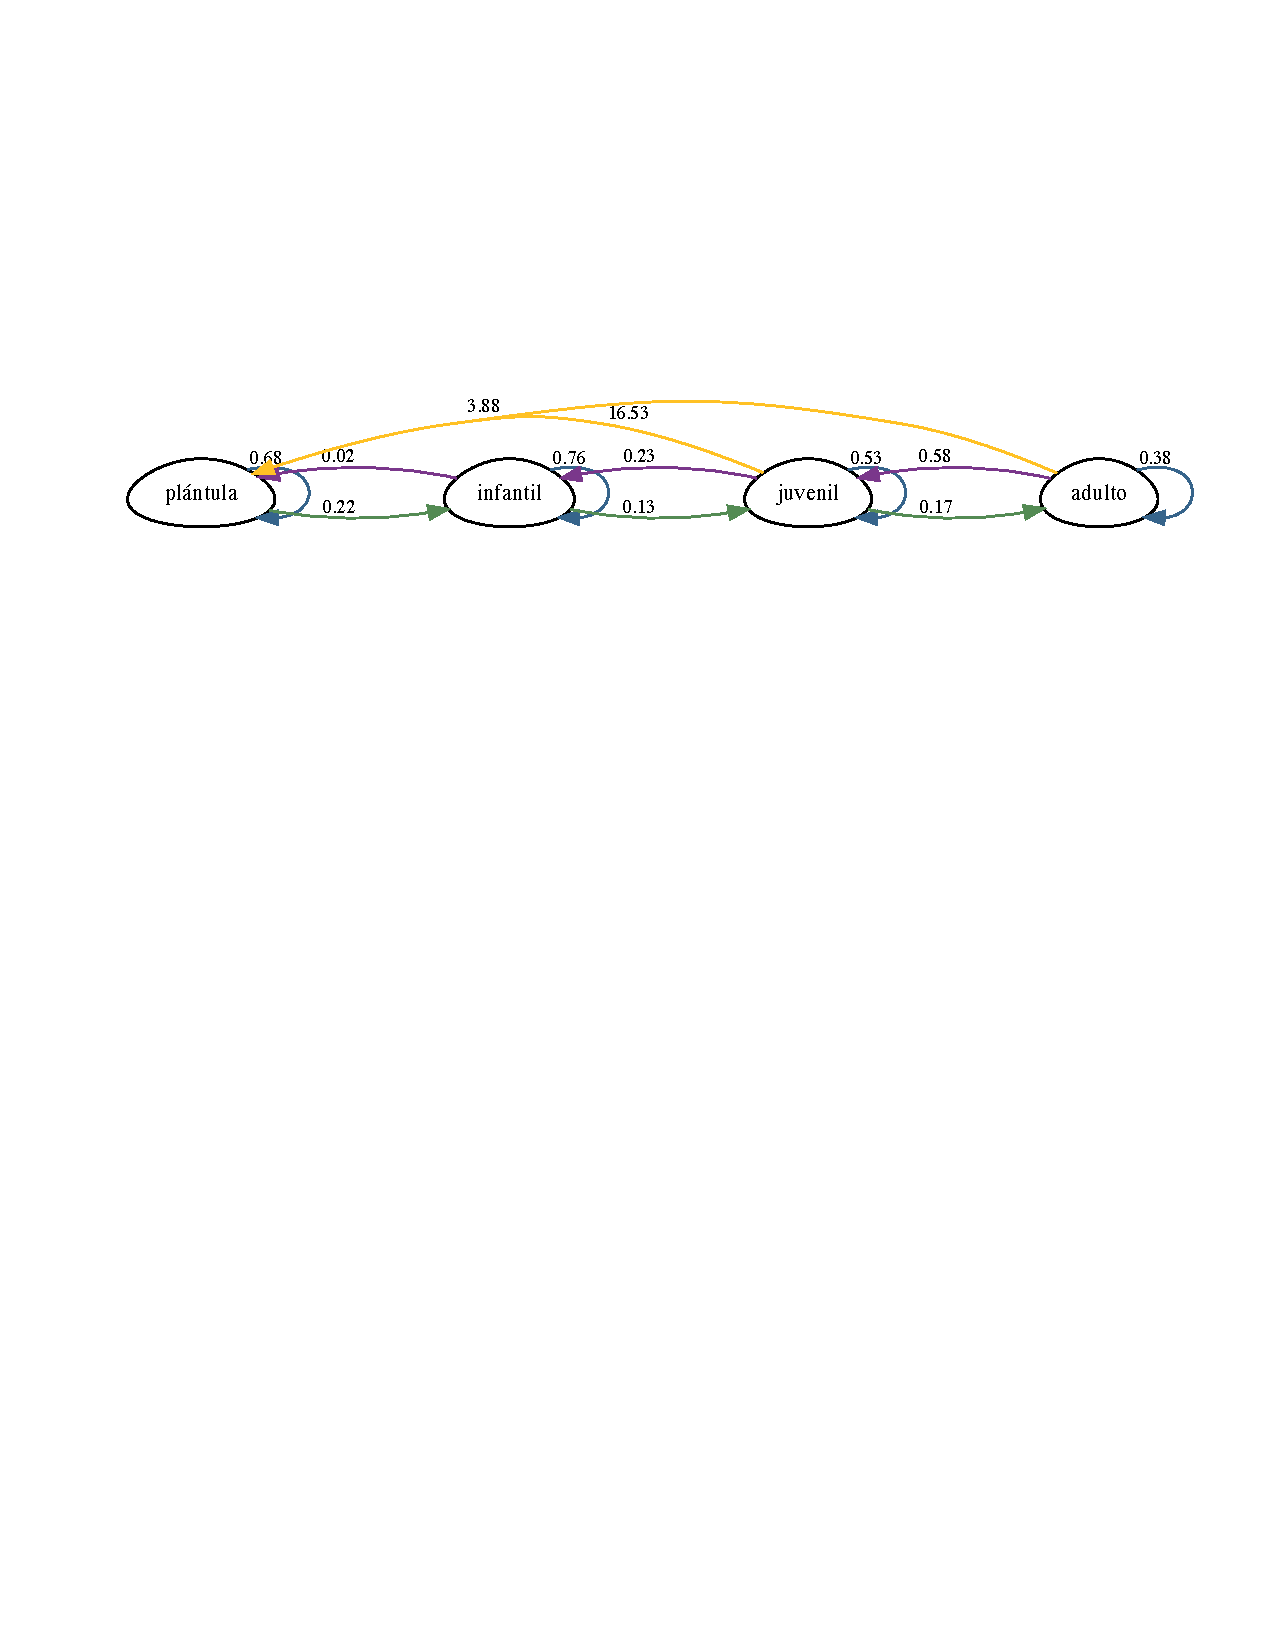
\includegraphics{114-LTRE_files/figure-pdf/LTRE2-1.pdf}

\vspace{-5truemm}

El ciclo de vida de \emph{Oncidium brachyandrum} creciendo sobre
\emph{Quercus martinezii}. Las flechas representan las transiciones
entre estadíos, estasis y fecundidades, y los números son las tasas
vitales de fecundidad, supervivencia y crecimiento. El color
\text{\textcolor[HTML]{FFC125}{amarillo}} para fecundidad,
\text{\textcolor[HTML]{36648B}{azul}} para supervivencia,
\text{\textcolor[HTML]{548B54}{verde}} para crecimiento,
\text{\textcolor[HTML]{7A378B}{violeta}} para retroceso y
\text{\textcolor[HTML]{36648B}{azul oscuro}} para permanencia.

\begin{center}\rule{0.5\linewidth}{0.5pt}\end{center}

\subsection{\texorpdfstring{Diagrama para \emph{Quercus
rugosa}}{Diagrama para Quercus rugosa}}\label{diagrama-para-quercus-rugosa}

\begin{Shaded}
\begin{Highlighting}[]
\NormalTok{matrug }\OtherTok{\textless{}{-}} \FunctionTok{rbind}\NormalTok{(}
  \FunctionTok{c}\NormalTok{(}\FloatTok{0.64}\NormalTok{, }\FloatTok{0.06}\NormalTok{, }\DecValTok{0}\NormalTok{, }\FloatTok{0.0045}\NormalTok{),}
  \FunctionTok{c}\NormalTok{(}\FloatTok{0.27}\NormalTok{, }\FloatTok{0.75}\NormalTok{, }\FloatTok{0.27}\NormalTok{, }\FloatTok{0.0}\NormalTok{),}
  \FunctionTok{c}\NormalTok{(}\FloatTok{0.0}\NormalTok{, }\FloatTok{0.08}\NormalTok{, }\FloatTok{0.47}\NormalTok{, }\FloatTok{0.28}\NormalTok{),}
  \FunctionTok{c}\NormalTok{(}\FloatTok{0.0}\NormalTok{, }\FloatTok{0.0}\NormalTok{, }\FloatTok{0.27}\NormalTok{, }\FloatTok{0.68}\NormalTok{))}


\NormalTok{stages }\OtherTok{\textless{}{-}} \FunctionTok{c}\NormalTok{(}\StringTok{"plántula"}\NormalTok{, }\StringTok{"infantil"}\NormalTok{, }\StringTok{"juvenil"}\NormalTok{, }\StringTok{"adulto"}\NormalTok{)}
\NormalTok{title }\OtherTok{\textless{}{-}} \ConstantTok{NULL}
\NormalTok{graph }\OtherTok{\textless{}{-}} \FunctionTok{expand.grid}\NormalTok{(}\AttributeTok{to =}\NormalTok{ stages, }\AttributeTok{from =}\NormalTok{ stages)}
\NormalTok{graph}\SpecialCharTok{$}\NormalTok{trans }\OtherTok{\textless{}{-}} \FunctionTok{round}\NormalTok{(}\FunctionTok{c}\NormalTok{(matrug), }\DecValTok{4}\NormalTok{)}
\NormalTok{graph }\OtherTok{\textless{}{-}}\NormalTok{ graph[graph}\SpecialCharTok{$}\NormalTok{trans }\SpecialCharTok{\textgreater{}} \DecValTok{0}\NormalTok{, ]}
\NormalTok{nodes }\OtherTok{\textless{}{-}} \FunctionTok{paste}\NormalTok{(}\FunctionTok{paste0}\NormalTok{(}\StringTok{"\textquotesingle{}"}\NormalTok{, stages, }\StringTok{"\textquotesingle{}"}\NormalTok{), }\AttributeTok{collapse =} \StringTok{"; "}\NormalTok{)}
\NormalTok{graph}\SpecialCharTok{$}\NormalTok{min\_len }\OtherTok{\textless{}{-}}\NormalTok{ (}\FunctionTok{as.numeric}\NormalTok{(graph}\SpecialCharTok{$}\NormalTok{to) }\SpecialCharTok{{-}} \FunctionTok{as.numeric}\NormalTok{(graph}\SpecialCharTok{$}\NormalTok{from)) }\SpecialCharTok{*} \DecValTok{4}
\NormalTok{graph}\SpecialCharTok{$}\NormalTok{col }\OtherTok{\textless{}{-}} \FunctionTok{c}\NormalTok{(}
\StringTok{"steelblue4"}\NormalTok{, }\StringTok{"PaleGreen4"}\NormalTok{, }\StringTok{"MediumOrchid4"}\NormalTok{, }\StringTok{"steelblue4"}\NormalTok{, }\StringTok{"PaleGreen4"}\NormalTok{, }\StringTok{"MediumOrchid4"}\NormalTok{,}\StringTok{"steelblue4"}\NormalTok{, }\StringTok{"PaleGreen4"}\NormalTok{,  }\StringTok{"Goldenrod1"}\NormalTok{, }\StringTok{"MediumOrchid4"}\NormalTok{, }\StringTok{"steelblue4"}
\NormalTok{)}
\NormalTok{edges }\OtherTok{\textless{}{-}} \FunctionTok{paste0}\NormalTok{(}\StringTok{"\textquotesingle{}"}\NormalTok{, graph}\SpecialCharTok{$}\NormalTok{from, }\StringTok{"\textquotesingle{}"}\NormalTok{, }\StringTok{" {-}\textgreater{} "}\NormalTok{, }\StringTok{"\textquotesingle{}"}\NormalTok{, graph}\SpecialCharTok{$}\NormalTok{to, }\StringTok{"\textquotesingle{}"}\NormalTok{,}
                \StringTok{"[minlen="}\NormalTok{, graph}\SpecialCharTok{$}\NormalTok{min\_len,}
                \StringTok{",fontsize="}\NormalTok{, }\DecValTok{10}\NormalTok{,}
                \StringTok{",color="}\NormalTok{, graph}\SpecialCharTok{$}\NormalTok{col,}
                \StringTok{",xlabel="}\NormalTok{, }\FunctionTok{paste}\NormalTok{(}\StringTok{"}\SpecialCharTok{\textbackslash{}"}\StringTok{"}\NormalTok{, graph}\SpecialCharTok{$}\NormalTok{trans),}
                \StringTok{"}\SpecialCharTok{\textbackslash{}"}\StringTok{]}\SpecialCharTok{\textbackslash{}n}\StringTok{"}\NormalTok{,}
                \AttributeTok{collapse =} \StringTok{""}
\NormalTok{)}
\FunctionTok{grViz}\NormalTok{(}
  \FunctionTok{paste}\NormalTok{(}
    \StringTok{"}
\StringTok{digraph \{}
\StringTok{  \{}
\StringTok{    graph[overlap=false];}
\StringTok{    rank=same;}
\StringTok{    node [shape="}\NormalTok{, }\StringTok{"egg"}\NormalTok{, }\StringTok{", fontsize="}\NormalTok{, }\DecValTok{12}\NormalTok{, }\StringTok{"];"}\NormalTok{,}
\NormalTok{    nodes, }\StringTok{"}
\StringTok{  \}"}\NormalTok{,}
    \StringTok{"ordering=out}
\StringTok{  x [style=invis]}
\StringTok{  x {-}\textgreater{} \{"}\NormalTok{, nodes, }\StringTok{"\} [style=invis]"}\NormalTok{, edges,}
    \StringTok{"labelloc=}\SpecialCharTok{\textbackslash{}"}\StringTok{t}\SpecialCharTok{\textbackslash{}"}\StringTok{;}
\StringTok{  label=}\SpecialCharTok{\textbackslash{}"}\StringTok{"}\NormalTok{, title, }\StringTok{"}\SpecialCharTok{\textbackslash{}"}
\StringTok{\}"}
\NormalTok{  )}
\NormalTok{)}
\end{Highlighting}
\end{Shaded}

\begin{verbatim}
file:////private/var/folders/3k/1ft37x9130vdbz21tw1497x40000gn/T/RtmpKH3tN8/file1090f357c360f/widget1090f6dc12e37.html screenshot completed
\end{verbatim}

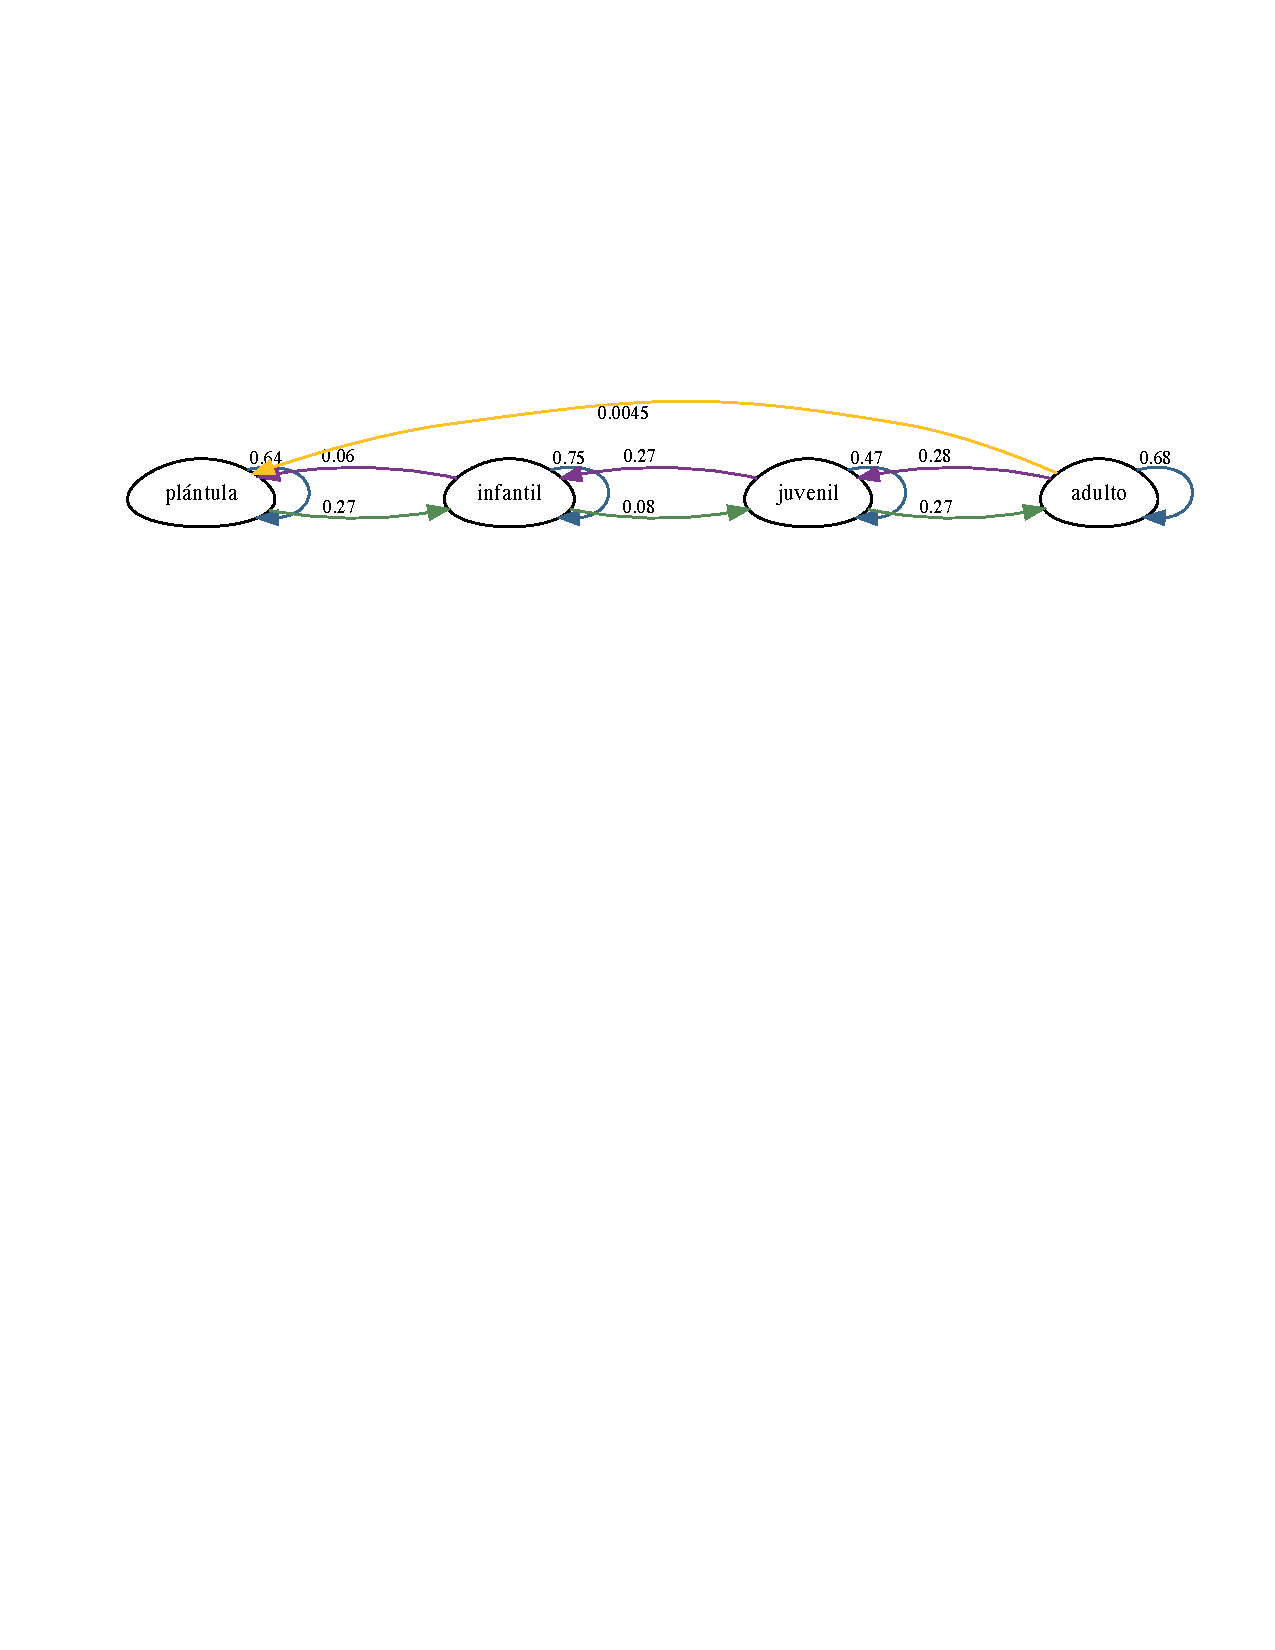
\includegraphics{114-LTRE_files/figure-pdf/LTRE3_Quercus_rugosa-1.pdf}

El ciclo de vida de \emph{Oncidium brachyandrum} creciendo sobre
\emph{Quercus rugosa}. Las flechas representan las transiciones entre
estadíos, estasis y fecundidades, y los números son las tasas vitales de
fecundidad, supervivencia y crecimiento. El color {amarillo} para
fecundidad, {azul} para supervivencia, {verde} para crecimiento,
{violeta} para retroceso y {azul oscuro} para permanencia.

\begin{center}\rule{0.5\linewidth}{0.5pt}\end{center}

\section{Procedimiento para ERTV en
Excel}\label{procedimiento-para-ertv-en-excel}

Para facilitar e entendimiento de cómo se calcula ERTV se creó la matriz
con los términos de referencia (Cuadro 1).

\begin{longtable}[]{@{}
  >{\raggedright\arraybackslash}p{(\columnwidth - 8\tabcolsep) * \real{0.2000}}
  >{\raggedright\arraybackslash}p{(\columnwidth - 8\tabcolsep) * \real{0.2000}}
  >{\raggedright\arraybackslash}p{(\columnwidth - 8\tabcolsep) * \real{0.2000}}
  >{\raggedright\arraybackslash}p{(\columnwidth - 8\tabcolsep) * \real{0.2000}}
  >{\raggedright\arraybackslash}p{(\columnwidth - 8\tabcolsep) * \real{0.2000}}@{}}
\toprule\noalign{}
\begin{minipage}[b]{\linewidth}\raggedright
Estadío
\end{minipage} & \begin{minipage}[b]{\linewidth}\raggedright
Plántulas (1)
\end{minipage} & \begin{minipage}[b]{\linewidth}\raggedright
Infantiles (2)
\end{minipage} & \begin{minipage}[b]{\linewidth}\raggedright
Juveniles (3)
\end{minipage} & \begin{minipage}[b]{\linewidth}\raggedright
Adultos (4)
\end{minipage} \\
\midrule\noalign{}
\endhead
\bottomrule\noalign{}
\endlastfoot
Plántulas (1) & p\textsubscript{11} (permanencia de plántulas) &
g\textsubscript{21} (retroceso de infantiles a plántulas) &
f\textsubscript{31} (plántulas generadas)g\textsubscript{31} (retroceso
de juveniles a plántulas) & f\textsubscript{41} (plántulas generadas) \\
Infantiles (2) & g\textsubscript{12} (crecimiento de plántulas a
infantiles) & p\textsubscript{22} (permanencia de infantiles) &
g\textsubscript{32} (retroceso de juveniles a infantiles) &
g\textsubscript{42} (retroceso de adultos a infantiles) \\
Juveniles (3) & g\textsubscript{13} (crecimiento de plántulas a
juveniles) & g\textsubscript{23} (crecimiento de infantiles a juveniles)
& p\textsubscript{33} (permanencia de juveniles) & g\textsubscript{43}
(retroceso de adultos a juveniles) \\
Adultos (4) & g\textsubscript{14} (crecimiento de plántulas a adultos) &
g\textsubscript{24} (crecimiento de infantiles a adultos) &
g\textsubscript{34} (crecimiento de juveniles a adultos) &
p\textsubscript{44} (permanencia de adultos) \\
Supervivencia & s\textsubscript{1} (de plántulas) & s\textsubscript{2}
(de infantiles) & s\textsubscript{3} (de juveniles) & s\textsubscript{4}
(de adultos) \\
\end{longtable}

\textbf{Cuadro 1.} Matriz de términos para el entendimiento de los ERTV.
Donde: f= fecundidad, g= crecimiento o retrogresión, p= permanencia y
s=supervivencia. Los subíndices se refieren a las transiciones entre
estadíos.Nota que los parámetros de juvenil que retrogresan a plántula y
esa etapa produciendo plántulas se suman.

En la sección \textbf{Apéndice C} se encuentra una hoja de Excel para
poder realizar los cálculos de ERTV. En esta sección se explica cómo se
construye la matriz de términos y cómo se calculan las tasas vitales
para cada una de las especies de hospedero.

Una vez colocadas las matrices en la hoja de trabajo el primer paso será
sumar las columnas para cada estadio, esto significará la supervivencia
(s) por estadío (s\textsubscript{1}, s\textsubscript{2},
s\textsubscript{3}, s\textsubscript{4}); para el caso de \emph{Q.
martinezii} en plántulas sería s\textsubscript{1}= 0.68+0.22= 0.90
(Figura 3). Después se tienen que calcular las transiciones con respecto
a la supervivencia; por lo que para el caso de la transición
g\textsubscript{12} para la matriz de \emph{Q. martinezii} tenemos
g\textsubscript{12}= 0.22/0.90=0.25; este cálculo se realiza para todas
las transiciones. Los valores de fecundidad (f) se tomarán tal cual de
la matriz de fecundidad \(matF\). Una vez obtenido esto se procederá a
realizar los cálculos con las ecuaciones que se muestran del lado
derecho para cada una de las celdas y, además, esto nos sirve para
verificar que hayamos calculado bien cada una de las tasas vitales. Por
ejemplo, observamos que una proporción de plántulas en \emph{Q.
martinezii} se mantuvo (0.67) este valor se obtiene de multiplicar la
supervivencia de plántulas (s\textsubscript{1}) por la sustracción de 1
menos el crecimiento de plántulas a infantiles 0.89 (1-0.25) = 0.68
(ecuación s\textsubscript{1}* (1-g\textsubscript{12})).

\begin{center}\rule{0.5\linewidth}{0.5pt}\end{center}

\subsection{Método usando Excel}\label{muxe9todo-usando-excel}

En un archivo nuevo de Excel se arma la base, con la columna de
vital\_rate al principio, seguido por las especies de hospederos
(tratamientos) poniendo primeramente el control y después la columna de
matrix. Esta base contendrá las ecuaciones de la matriz de referencia.
Como la matriz de \emph{Q. martinezii} tuvo los valores más altos de
lambda está se colocará primero en nuestra base que utilizaremos para
correr el análisis ERTV.

\begin{table}
\fontsize{12.0pt}{14.0pt}\selectfont
\begin{tabular*}{\linewidth}{@{\extracolsep{\fill}}lrrl}
\toprule
names.vitalrate & martinezzi & rugosa & matrix \\ 
\midrule\addlinespace[2.5pt]
lambda & 1.30000000 & 0.9300000 &  \\ 
s1 & 0.89610000 & 0.8636000 & s1*(1-g12) \\ 
g12 & 0.24637681 & 0.2631579 & s1*g12 \\ 
s2 & 0.90163934 & 0.8888889 & 0 \\ 
g21 & 0.01818182 & 0.0625000 & 0 \\ 
g23 & 0.14545450 & 0.0937499 & s2*g21 \\ 
s3 & 0.93750000 & 0.9999900 & s2*(1-g23-g21) \\ 
g32 & 0.25000000 & 0.2666670 & s2*g23 \\ 
g34 & 0.18333300 & 0.2666670 & 0 \\ 
s4 & 0.96666700 & 0.9545455 & f31 \\ 
g43 & 0.60344800 & 0.2857140 & s3*g32 \\ 
f31 & 3.87500000 & 0.0001000 & s3*(1-g34-g32) \\ 
f41 & 16.53000000 & 0.0045000 & s3*g34 \\ 
NA & NA & NA & f41 \\ 
NA & NA & NA & 0 \\ 
NA & NA & NA & s4*g43 \\ 
NA & NA & NA & s4*(1-g43) \\ 
\bottomrule
\end{tabular*}
\end{table}

\textbf{Cuadro 2.} Ejemplo de base para poder calcular los ERTV.

Es importante colocar en la segunda fila la palabra lambda en la primera
columna y después los valores según corresponda a cada tratamiento.
Debido a que en \emph{Q. rugosa} no hubo producción de plántulas
(f\textsubscript{31}) pero en \emph{Q. martinezii} si hubo se coloca una
cantidad muy pequeña pero mayor a cero (e.g.~0.00001) para que se pueda
correr el análisis, para las otras transiciones en valor puede ser 0.
Una vez culminada la base se guarda el archivo en formato de texto, para
continuar en R. Es importante comenzar a colocar las ecuaciones a partir
de la segunda fila en la columna matrix.

\begin{center}\rule{0.5\linewidth}{0.5pt}\end{center}

\section{Procedimiento en R}\label{procedimiento-en-r}

Subir la base de datos de la carpeta de trabajo y cargarla en R.

\begin{itemize}
\tightlist
\item
  Nota que debería observar la base de datos en la consola de R para
  verificar que se haya cargado correctamente con los mismos valores que
  en la hoja de Excel.
\end{itemize}

\begin{Shaded}
\begin{Highlighting}[]
\CommentTok{\# Asegurarse de tener instalado y cargado el paquete \textquotesingle{}popbio\textquotesingle{} package }

\CommentTok{\# oncidium\textless{}{-}read.table("data/vitalratesoncidium.txt", sep="\textbackslash{}t", header=TRUE, stringsAsFactors=FALSE, fill=TRUE) }
     \CommentTok{\# Aqui la alternativa si tiene los datos en una hoja de Excel}

\CommentTok{\#oncidium }

\NormalTok{Oncidium}
\end{Highlighting}
\end{Shaded}

\begin{verbatim}
# A tibble: 17 x 4
   names.vitalrate martinezzi  rugosa matrix          
   <chr>                <dbl>   <dbl> <chr>           
 1 lambda              1.3     0.93   ""              
 2 s1                  0.896   0.864  "s1*(1-g12)"    
 3 g12                 0.246   0.263  "s1*g12"        
 4 s2                  0.902   0.889  "0"             
 5 g21                 0.0182  0.0625 "0"             
 6 g23                 0.145   0.0937 "s2*g21"        
 7 s3                  0.938   1.000  "s2*(1-g23-g21)"
 8 g32                 0.25    0.267  "s2*g23"        
 9 g34                 0.183   0.267  "0"             
10 s4                  0.967   0.955  "f31"           
11 g43                 0.603   0.286  "s3*g32"        
12 f31                 3.88    0.0001 "s3*(1-g34-g32)"
13 f41                16.5     0.0045 "s3*g34"        
14 <NA>               NA      NA      "f41"           
15 <NA>               NA      NA      "0"             
16 <NA>               NA      NA      "s4*g43"        
17 <NA>               NA      NA      "s4*(1-g43)"    
\end{verbatim}

Debido a que la columna de matriz contiene más filas con datos nos
aparecerá la leyenda NA en las otras columnas esto se refiere a que no
hay valores disponibles para esas filas

Para extraer los nombres de las tasas vitales (de la fila 2 a la 13),
sin incluir el valor de \(\lambda\) el cual está en la primera

\begin{Shaded}
\begin{Highlighting}[]
\NormalTok{razonvital }\OtherTok{\textless{}{-}}\NormalTok{ Oncidium}\SpecialCharTok{$}\NormalTok{names.vitalrate[}\DecValTok{2}\SpecialCharTok{:}\DecValTok{13}\NormalTok{]}

\NormalTok{razonvital }\CommentTok{\# mostrar los nombres del objeto razón vital}
\end{Highlighting}
\end{Shaded}

\begin{verbatim}
 [1] "s1"  "g12" "s2"  "g21" "g23" "s3"  "g32" "g34" "s4"  "g43" "f31" "f41"
\end{verbatim}

\begin{center}\rule{0.5\linewidth}{0.5pt}\end{center}

\subsection{\texorpdfstring{Tasa vital sobre \emph{Q.
martinezzi}}{Tasa vital sobre Q. martinezzi}}\label{tasa-vital-sobre-q.-martinezzi}

Extraer tasas vitales de de la orquídea \emph{Oncidium brachyandrum} que
crecen sobre \emph{Q. martinezzi} y dejar a lambda a un lado

\begin{Shaded}
\begin{Highlighting}[]
\NormalTok{Martinezzi }\OtherTok{\textless{}{-}}\NormalTok{ Oncidium}\SpecialCharTok{$}\NormalTok{martinezzi[}\DecValTok{2}\SpecialCharTok{:}\DecValTok{13}\NormalTok{] }\CommentTok{\# [2:13] se refiere a la fila 2 hasta la 13.}
\FunctionTok{names}\NormalTok{(Martinezzi) }\OtherTok{\textless{}{-}}\NormalTok{ razonvital }\CommentTok{\# asignar los nombres de las tasas vitales}
\NormalTok{Martinezzi}
\end{Highlighting}
\end{Shaded}

\begin{verbatim}
         s1         g12          s2         g21         g23          s3 
 0.89610000  0.24637681  0.90163934  0.01818182  0.14545450  0.93750000 
        g32         g34          s4         g43         f31         f41 
 0.25000000  0.18333300  0.96666700  0.60344800  3.87500000 16.53000000 
\end{verbatim}

\begin{center}\rule{0.5\linewidth}{0.5pt}\end{center}

\subsection{\texorpdfstring{Tasa vital sobre \emph{Q.
rugosa}}{Tasa vital sobre Q. rugosa}}\label{tasa-vital-sobre-q.-rugosa}

Extraer tasas vitales de de la orquidea \emph{Oncidium brachyandrum} que
crecen sobre \emph{Q. rugosa} y dejar a lambda a un lado

\begin{Shaded}
\begin{Highlighting}[]
\NormalTok{Rugosa }\OtherTok{\textless{}{-}}\NormalTok{ Oncidium}\SpecialCharTok{$}\NormalTok{rugosa[}\DecValTok{2}\SpecialCharTok{:}\DecValTok{13}\NormalTok{]}
\FunctionTok{names}\NormalTok{(Rugosa) }\OtherTok{\textless{}{-}}\NormalTok{ razonvital }\CommentTok{\# asignar los nombres de las tasas vitales}
\NormalTok{Rugosa}
\end{Highlighting}
\end{Shaded}

\begin{verbatim}
       s1       g12        s2       g21       g23        s3       g32       g34 
0.8636000 0.2631579 0.8888889 0.0625000 0.0937499 0.9999900 0.2666670 0.2666670 
       s4       g43       f31       f41 
0.9545455 0.2857140 0.0001000 0.0045000 
\end{verbatim}

\subsection{Extraer los elementos de matriz utilizando los nombres de
las tasas
vitales}\label{extraer-los-elementos-de-matriz-utilizando-los-nombres-de-las-tasas-vitales}

\begin{Shaded}
\begin{Highlighting}[]
\NormalTok{matrix.el}\OtherTok{\textless{}{-}}\FunctionTok{as.expression}\NormalTok{(}\FunctionTok{parse}\NormalTok{(}\AttributeTok{text=}\NormalTok{Oncidium}\SpecialCharTok{$}\NormalTok{matrix)) }
\NormalTok{matrix.el}
\end{Highlighting}
\end{Shaded}

\begin{verbatim}
expression(s1 * (1 - g12), s1 * g12, 0, 0, s2 * g21, s2 * (1 - 
    g23 - g21), s2 * g23, 0, f31, s3 * g32, s3 * (1 - g34 - g32), 
    s3 * g34, f41, 0, s4 * g43, s4 * (1 - g43))
\end{verbatim}

\begin{Shaded}
\begin{Highlighting}[]
\FunctionTok{expression}\NormalTok{(s1}\SpecialCharTok{*}\NormalTok{(}\DecValTok{1}\SpecialCharTok{{-}}\NormalTok{g12), s1}\SpecialCharTok{*}\NormalTok{g12, }\DecValTok{0}\NormalTok{, }\DecValTok{0}\NormalTok{, }
\NormalTok{           s2}\SpecialCharTok{*}\NormalTok{g21, s2}\SpecialCharTok{*}\NormalTok{(}\DecValTok{1}\SpecialCharTok{{-}}\NormalTok{g23}\SpecialCharTok{{-}}\NormalTok{g21), s2}\SpecialCharTok{*}\NormalTok{g23, }\DecValTok{0}\NormalTok{, }
\NormalTok{          f31, s3}\SpecialCharTok{*}\NormalTok{g32, s3}\SpecialCharTok{*}\NormalTok{(}\DecValTok{1}\SpecialCharTok{{-}}\NormalTok{g34}\SpecialCharTok{{-}}\NormalTok{g32), s3}\SpecialCharTok{*}\NormalTok{g34, }
\NormalTok{          f41, }\DecValTok{0}\NormalTok{, s4}\SpecialCharTok{*}\NormalTok{g43, s4}\SpecialCharTok{*}\NormalTok{(}\DecValTok{1}\SpecialCharTok{{-}}\NormalTok{g43))}
\end{Highlighting}
\end{Shaded}

\begin{verbatim}
expression(s1 * (1 - g12), s1 * g12, 0, 0, s2 * g21, s2 * (1 - 
    g23 - g21), s2 * g23, 0, f31, s3 * g32, s3 * (1 - g34 - g32), 
    s3 * g34, f41, 0, s4 * g43, s4 * (1 - g43))
\end{verbatim}

\subsection{\texorpdfstring{Calcular las sensibilidades y elasticidades
del ERTV para cada una de las matrices de \emph{Oncidium
brachyandrum}}{Calcular las sensibilidades y elasticidades del ERTV para cada una de las matrices de Oncidium brachyandrum}}\label{calcular-las-sensibilidades-y-elasticidades-del-ertv-para-cada-una-de-las-matrices-de-oncidium-brachyandrum}

Nota que usando la función vitalsens se pueden calcular las
sensibilidades y elasticidades de las tasas vitales de las matrices de
\emph{Oncidium brachyandrum} creciendo sobre \emph{Q. martinezii} y
\emph{Q. rugosa} en un mismo objeto.

\subsubsection{\texorpdfstring{\emph{Quercus
matinezzi}}{Quercus matinezzi}}\label{quercus-matinezzi}

\begin{Shaded}
\begin{Highlighting}[]
\NormalTok{Martinezzi.se }\OtherTok{\textless{}{-}} \FunctionTok{vitalsens}\NormalTok{(matrix.el, Martinezzi)}

\NormalTok{Martinezzi.se }\CommentTok{\# observar los resultados}
\end{Highlighting}
\end{Shaded}

\begin{verbatim}
       estimate  sensitivity   elasticity
s1   0.89610000  0.391848564  0.270331597
g12  0.24637681  0.441970792  0.083833089
s2   0.90163934  0.487546981  0.338431982
g21  0.01818182 -0.197108462 -0.002759082
g23  0.14545450  0.948968500  0.106267639
s3   0.93750000  0.285323303  0.205935203
g32  0.25000000 -0.196618688 -0.037843115
g34  0.18333300  0.309836570  0.043731603
s4   0.96666700  0.076632964  0.057031473
g43  0.60344800 -0.059973210 -0.027862445
f31  3.87500000  0.023876282  0.071229597
f41 16.53000000  0.004482143  0.057040147
\end{verbatim}

\subsubsection{\texorpdfstring{\emph{Quercus
rugosa}}{Quercus rugosa}}\label{quercus-rugosa}

\begin{Shaded}
\begin{Highlighting}[]
\FunctionTok{elas}\NormalTok{(matrug)}
\end{Highlighting}
\end{Shaded}

\begin{verbatim}
           [,1]       [,2]       [,3]         [,4]
[1,] 0.04605361 0.02046105 0.00000000 0.0007706189
[2,] 0.02123167 0.27949530 0.04773035 0.0000000000
[3,] 0.00000000 0.04850097 0.13516864 0.0852450199
[4,] 0.00000000 0.00000000 0.08601564 0.2293271456
\end{verbatim}

\begin{Shaded}
\begin{Highlighting}[]
\NormalTok{Rugosa.se}\OtherTok{\textless{}{-}}\FunctionTok{vitalsens}\NormalTok{(matrix.el, Rugosa)}
\NormalTok{Rugosa.se}
\end{Highlighting}
\end{Shaded}

\begin{verbatim}
     estimate sensitivity    elasticity
s1  0.8636000  0.05650198  5.255855e-02
g12 0.2631579  0.01294108  3.668208e-03
s2  0.8888889  0.35500473  3.398981e-01
g21 0.0625000 -0.06703010 -4.512498e-03
g23 0.0937499  0.18792055  1.897633e-02
s3  0.9999900  0.25571734  2.754374e-01
g32 0.2666670 -0.10562652 -3.033956e-02
g34 0.2666670  0.03162376  9.083430e-03
s4  0.9545455  0.32232024  3.313991e-01
g43 0.2857140 -0.03264579 -1.004675e-02
f31 0.0001000  0.13214735  1.423395e-05
f41 0.0045000  0.14291279  6.927088e-04
\end{verbatim}

\subsection{Calcular las diferencias en tasas vitales entre las especies
de
hospederos}\label{calcular-las-diferencias-en-tasas-vitales-entre-las-especies-de-hospederos}

En esta parte se calculará la diferencia entre las tasas vitales de
\emph{Oncidium brachyandrum} creciendo sobre \emph{Q. martinezii} y
\emph{Q. rugosa}. ¿Como se interpreta estos resultados?

\begin{Shaded}
\begin{Highlighting}[]
\NormalTok{vr.dif.Martinezzi.Rugosa }\OtherTok{\textless{}{-}}\NormalTok{ Rugosa }\SpecialCharTok{{-}}\NormalTok{ Martinezzi}
\NormalTok{vr.dif.Martinezzi.Rugosa}
\end{Highlighting}
\end{Shaded}

\begin{verbatim}
          s1          g12           s2          g21          g23           s3 
 -0.03250000   0.01678109  -0.01275045   0.04431819  -0.05170460   0.06249000 
         g32          g34           s4          g43          f31          f41 
  0.01666700   0.08333400  -0.01212155  -0.31773400  -3.87490000 -16.52550000 
\end{verbatim}

\subsection{Calcular las tasas vitales para la matriz
media}\label{calcular-las-tasas-vitales-para-la-matriz-media}

En este paso se calculará la tasa vital media para \emph{Oncidium
brachyandrum} creciendo sobre \emph{Q. martinezii} y \emph{Q. rugosa}.
La tasa vital media se calcula sumando las tasas vitales de las dos
matrices y dividiendo entre 2.

\begin{Shaded}
\begin{Highlighting}[]
\NormalTok{vr.promedia.Martinezzi.Rugosa }\OtherTok{\textless{}{-}}\NormalTok{ ((Rugosa }\SpecialCharTok{+}\NormalTok{ Martinezzi) }\SpecialCharTok{/} \DecValTok{2}\NormalTok{) }\CommentTok{\#calcular la tazas vitales parta la matrix promedia}

\CommentTok{\# Nota: si se tuvieran 3 matrices se sumarían las tasas vitales de las tres dividido por 3.}

\NormalTok{vr.promedia.Martinezzi.Rugosa}
\end{Highlighting}
\end{Shaded}

\begin{verbatim}
        s1        g12         s2        g21        g23         s3        g32 
0.87985000 0.25476735 0.89526412 0.04034091 0.11960220 0.96874500 0.25833350 
       g34         s4        g43        f31        f41 
0.22500000 0.96060623 0.44458100 1.93755000 8.26725000 
\end{verbatim}

\subsection{Calcular las tasas sensibilidades y elasticidades para la
matriz
media}\label{calcular-las-tasas-sensibilidades-y-elasticidades-para-la-matriz-media}

En este paso se calculará las sensibilidades y elasticidades para la
matriz promedia de \emph{Oncidium brachyandrum} creciendo sobre \emph{Q.
martinezii} y \emph{Q. rugosa}.

\begin{Shaded}
\begin{Highlighting}[]
\NormalTok{media.sens.Martinezzi.Rugosa }\OtherTok{\textless{}{-}} \FunctionTok{vitalsens}\NormalTok{(}
\NormalTok{  matrix.el,}
\NormalTok{  vr.promedia.Martinezzi.Rugosa}
\NormalTok{)}
\NormalTok{media.sens.Martinezzi.Rugosa}
\end{Highlighting}
\end{Shaded}

\begin{verbatim}
      estimate  sensitivity  elasticity
s1  0.87985000  0.329916405  0.24324014
g12 0.25476735  0.299340210  0.06390451
s2  0.89526412  0.443898046  0.33300987
g21 0.04034091 -0.173842318 -0.00587657
g23 0.11960220  0.888672313  0.08906427
s3  0.96874500  0.263014361  0.21350676
g32 0.25833350 -0.186604631 -0.04039483
g34 0.22500000  0.239081436  0.04507659
s4  0.96060623  0.130258448  0.10485134
g43 0.44458100 -0.078313577 -0.02917499
f31 1.93755000  0.026940498  0.04374025
f41 8.26725000  0.008899404  0.06165164
\end{verbatim}

\subsection{Calcular las contribuciones de ERTV y ver los
resultados}\label{calcular-las-contribuciones-de-ertv-y-ver-los-resultados}

\begin{Shaded}
\begin{Highlighting}[]
\NormalTok{LTRE.contrib.Martinezzi.Rugosa }\OtherTok{\textless{}{-}}\NormalTok{ vr.dif.Martinezzi.Rugosa }\SpecialCharTok{*}
\NormalTok{  media.sens.Martinezzi.Rugosa}\SpecialCharTok{$}\NormalTok{sensitivity}
\NormalTok{LTRE.contrib.Martinezzi.Rugosa}
\end{Highlighting}
\end{Shaded}

\begin{verbatim}
          s1          g12           s2          g21          g23           s3 
-0.010722283  0.005023254 -0.005659900 -0.007704377 -0.045948446  0.016435767 
         g32          g34           s4          g43          f31          f41 
-0.003110139  0.019923612 -0.001578934  0.024882886 -0.104391736 -0.147067093 
\end{verbatim}

\subsection{Resultados de ERTV}\label{resultados-de-ertv}

En esta sección se une todos los resultados en un solo objeto para poder
observarlos de manera conjunta.

\begin{Shaded}
\begin{Highlighting}[]
\NormalTok{LTRE.resultados.Martinezzi.Rugosa }\OtherTok{\textless{}{-}} \FunctionTok{data.frame}\NormalTok{(}
  \AttributeTok{razonvital =}\NormalTok{ razonvital,}
  \AttributeTok{rug.vr =}\NormalTok{ Rugosa,}
  \AttributeTok{mart.vr =}\NormalTok{ Martinezzi,}
  \AttributeTok{vr.differencia =}\NormalTok{ vr.dif.Martinezzi.Rugosa,}
  \AttributeTok{media.sens =}\NormalTok{ media.sens.Martinezzi.Rugosa}\SpecialCharTok{$}\NormalTok{sensitivity,}
  \AttributeTok{contribucion =}\NormalTok{ LTRE.contrib.Martinezzi.Rugosa}
\NormalTok{)}

\FunctionTok{gt}\NormalTok{(LTRE.resultados.Martinezzi.Rugosa)}
\end{Highlighting}
\end{Shaded}

\begin{table}
\fontsize{12.0pt}{14.0pt}\selectfont
\begin{tabular*}{\linewidth}{@{\extracolsep{\fill}}lrrrrr}
\toprule
razonvital & rug.vr & mart.vr & vr.differencia & media.sens & contribucion \\ 
\midrule\addlinespace[2.5pt]
s1 & 0.8636000 & 0.89610000 & -0.03250000 & 0.329916405 & -0.010722283 \\ 
g12 & 0.2631579 & 0.24637681 & 0.01678109 & 0.299340210 & 0.005023254 \\ 
s2 & 0.8888889 & 0.90163934 & -0.01275045 & 0.443898046 & -0.005659900 \\ 
g21 & 0.0625000 & 0.01818182 & 0.04431819 & -0.173842318 & -0.007704377 \\ 
g23 & 0.0937499 & 0.14545450 & -0.05170460 & 0.888672313 & -0.045948446 \\ 
s3 & 0.9999900 & 0.93750000 & 0.06249000 & 0.263014361 & 0.016435767 \\ 
g32 & 0.2666670 & 0.25000000 & 0.01666700 & -0.186604631 & -0.003110139 \\ 
g34 & 0.2666670 & 0.18333300 & 0.08333400 & 0.239081436 & 0.019923612 \\ 
s4 & 0.9545455 & 0.96666700 & -0.01212155 & 0.130258448 & -0.001578934 \\ 
g43 & 0.2857140 & 0.60344800 & -0.31773400 & -0.078313577 & 0.024882886 \\ 
f31 & 0.0001000 & 3.87500000 & -3.87490000 & 0.026940498 & -0.104391736 \\ 
f41 & 0.0045000 & 16.53000000 & -16.52550000 & 0.008899404 & -0.147067093 \\ 
\bottomrule
\end{tabular*}
\end{table}

\begin{center}\rule{0.5\linewidth}{0.5pt}\end{center}

\subsection{Graficar los resultados de
ERTV}\label{graficar-los-resultados-de-ertv}

Se puede crear un gráfico de la contribución de cada tasa vitales sobre
la historia de vida de la especies comparando las dos matrix

\begin{Shaded}
\begin{Highlighting}[]
\FunctionTok{ggplot}\NormalTok{(}
\NormalTok{  LTRE.resultados.Martinezzi.Rugosa,}
  \FunctionTok{aes}\NormalTok{(}\AttributeTok{y =}\NormalTok{ contribucion, }\AttributeTok{x =}\NormalTok{ razonvital, }\AttributeTok{fill =}\NormalTok{ razonvital)}
\NormalTok{) }\SpecialCharTok{+}
  \FunctionTok{geom\_bar}\NormalTok{(}\AttributeTok{stat =} \StringTok{"identity"}\NormalTok{) }\SpecialCharTok{+}
  \FunctionTok{rlt\_style\_fill}\NormalTok{() }\SpecialCharTok{+}
  \FunctionTok{theme}\NormalTok{(}\AttributeTok{axis.text.x =} \FunctionTok{element\_text}\NormalTok{(}\AttributeTok{angle =} \DecValTok{90}\NormalTok{, }\AttributeTok{hjust =} \DecValTok{1}\NormalTok{)) }\SpecialCharTok{+}
  \FunctionTok{labs}\NormalTok{(}
    \AttributeTok{title =} \StringTok{"Oncidium vital rate contribución a la diferencia en lambda"}\NormalTok{,}
    \AttributeTok{x =} \StringTok{"razonvital"}\NormalTok{,}
    \AttributeTok{y =} \StringTok{"contribución"}
\NormalTok{  ) }\SpecialCharTok{+}
  \FunctionTok{geom\_hline}\NormalTok{(}\AttributeTok{yintercept =} \DecValTok{0}\NormalTok{, }\AttributeTok{linetype =} \StringTok{"dashed"}\NormalTok{, }\AttributeTok{color =} \StringTok{"red"}\NormalTok{) }\SpecialCharTok{+}
  \FunctionTok{xlab}\NormalTok{(}\StringTok{"Tasa vitales"}\NormalTok{)}
\end{Highlighting}
\end{Shaded}

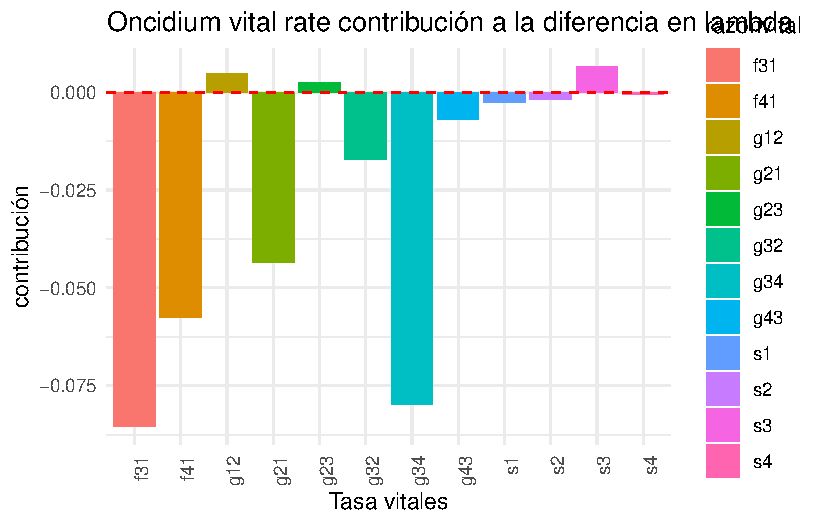
\includegraphics{114-LTRE_files/figure-pdf/LTRE15-1.pdf}

Figure 5. Resultados de un Experimento de Respuesta de la Tabla de Vida
(ERTV) llevado a cabo para evaluar las contribuciones de las entradas de
la matriz a la variación observada en \emph{λ}.

De acuerdo con el análisis de elasticidad para cada una de las
poblaciones de \emph{O. brachyandrum}, tanto en \emph{Q. martinezii}
como en \emph{Q. rugosa} la permanencia de individuos infantiles es la
que tiene un mayor impacto sobre los valores de la tasa de crecimiento
poblacional (Figura 6). De acuerdo al ERTV, el cual toma en cuenta las
diferencias en las tasas vitales y la sensibilidad de lambda que es una
función no linear de esas tasas vitales, podemos observar que la
fecundidad (\(f_{sa}\)) y el crecimiento de plántulas a juveniles
(\(g_{sj}\)), de juveniles a adultos (\(g_{ja}\)) y el retroceso de
adultos a juveniles (\(g_{aj}\)) tiene las mayores contribuciones a las
diferencias en lambda entre \emph{Q. martinezii} y \emph{Q. rugosa} que
la permanencia de plántulas.

Figure 6. Resultados de los análisis de elasticidad, para dos
poblaciones de \emph{Oncidium brachyandrum} creciendo sobre
\emph{Quercus martinezii} y \emph{Q. rugosa}. Por proceso demográfico
(a) y por estadío (b).

\begin{Shaded}
\begin{Highlighting}[]
\FunctionTok{ggplot}\NormalTok{(}
\NormalTok{  LTRE.resultados.Martinezzi.Rugosa,}
  \FunctionTok{aes}\NormalTok{(}\AttributeTok{y =}\NormalTok{ media.sens, }\AttributeTok{x =}\NormalTok{ razonvital, }\AttributeTok{fill =}\NormalTok{ razonvital)}
\NormalTok{) }\SpecialCharTok{+}
  \FunctionTok{geom\_bar}\NormalTok{(}\AttributeTok{stat =} \StringTok{"identity"}\NormalTok{) }\SpecialCharTok{+}
  \FunctionTok{rlt\_style\_fill}\NormalTok{() }\SpecialCharTok{+}
  \FunctionTok{theme}\NormalTok{(}\AttributeTok{axis.text.x =} \FunctionTok{element\_text}\NormalTok{(}\AttributeTok{angle =} \DecValTok{90}\NormalTok{, }\AttributeTok{hjust =} \DecValTok{1}\NormalTok{)) }\SpecialCharTok{+}
  \FunctionTok{labs}\NormalTok{(}
    \AttributeTok{title =} \StringTok{"Promedio de la Sensitividad"}\NormalTok{,}
    \AttributeTok{x =} \StringTok{"razonvital"}\NormalTok{,}
    \AttributeTok{y =} \StringTok{"contribución"}
\NormalTok{  ) }\SpecialCharTok{+}
  \FunctionTok{geom\_hline}\NormalTok{(}\AttributeTok{yintercept =} \DecValTok{0}\NormalTok{, }\AttributeTok{linetype =} \StringTok{"dashed"}\NormalTok{, }\AttributeTok{color =} \StringTok{"red"}\NormalTok{) }\SpecialCharTok{+}
  \FunctionTok{xlab}\NormalTok{(}\StringTok{"Tasa vitales"}\NormalTok{)}
\end{Highlighting}
\end{Shaded}

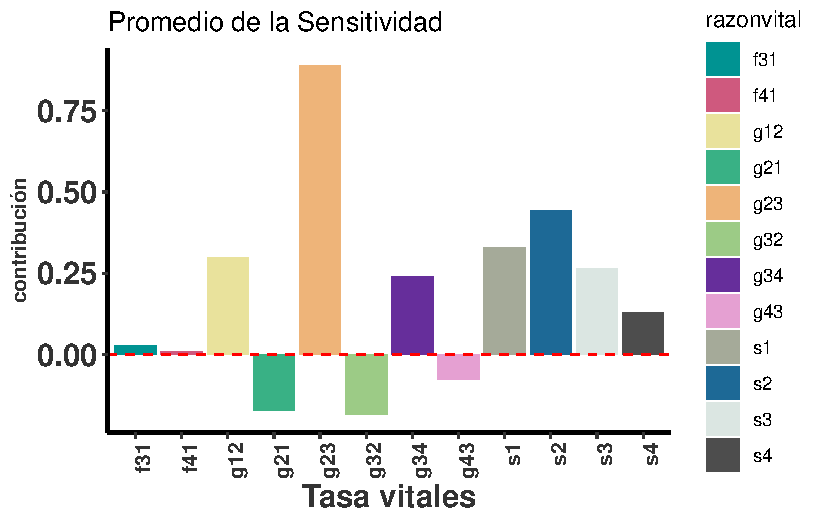
\includegraphics{114-LTRE_files/figure-pdf/LTRE16-1.pdf}

\begin{center}\rule{0.5\linewidth}{0.5pt}\end{center}

\section{Análisis con R}\label{anuxe1lisis-con-r}

Ahora enseñar como hacer estos análisis sin tener que usar Excel, aquí
un set de script para aplicar a \emph{Oncidium brachyandrum}.

\begin{center}\rule{0.5\linewidth}{0.5pt}\end{center}

En esta sección se muestra cómo hacer los análisis de ERTV sin tener que
usar Excel, utilizando directamente R. Esto es útil para evitar los
pasos intermedios y realizar el análisis de manera más eficiente.

Calcular la matriz promedio

\begin{Shaded}
\begin{Highlighting}[]
\NormalTok{mat.promedio }\OtherTok{\textless{}{-}}\NormalTok{ (matmart }\SpecialCharTok{+}\NormalTok{ matrug) }\SpecialCharTok{/} \DecValTok{2}

\NormalTok{mat.promedio}
\end{Highlighting}
\end{Shaded}

\begin{verbatim}
      [,1]  [,2] [,3]    [,4]
[1,] 0.660 0.040 1.94 8.26725
[2,] 0.245 0.755 0.25 0.00000
[3,] 0.000 0.105 0.50 0.43000
[4,] 0.000 0.000 0.22 0.53000
\end{verbatim}

\section{Convertir las matrices en un
vectores}\label{convertir-las-matrices-en-un-vectores}

\begin{Shaded}
\begin{Highlighting}[]
\NormalTok{mat.promedio.vector }\OtherTok{\textless{}{-}} \FunctionTok{as.vector}\NormalTok{(mat.promedio)}

\NormalTok{mat.promedio.vector}
\end{Highlighting}
\end{Shaded}

\begin{verbatim}
 [1] 0.66000 0.24500 0.00000 0.00000 0.04000 0.75500 0.10500 0.00000 1.94000
[10] 0.25000 0.50000 0.22000 8.26725 0.00000 0.43000 0.53000
\end{verbatim}

\begin{Shaded}
\begin{Highlighting}[]
\NormalTok{mat\_rug.vector }\OtherTok{\textless{}{-}} \FunctionTok{as.vector}\NormalTok{(matrug) }\CommentTok{\# vector para O. rugosa}
\NormalTok{mat\_mart.vector }\OtherTok{\textless{}{-}} \FunctionTok{as.vector}\NormalTok{(matmart) }\CommentTok{\# vector para O. martinezii}
\end{Highlighting}
\end{Shaded}

\begin{Shaded}
\begin{Highlighting}[]
\NormalTok{mat\_rug.vector}
\end{Highlighting}
\end{Shaded}

\begin{verbatim}
 [1] 0.6400 0.2700 0.0000 0.0000 0.0600 0.7500 0.0800 0.0000 0.0000 0.2700
[11] 0.4700 0.2700 0.0045 0.0000 0.2800 0.6800
\end{verbatim}

\begin{Shaded}
\begin{Highlighting}[]
\NormalTok{matrug}
\end{Highlighting}
\end{Shaded}

\begin{verbatim}
     [,1] [,2] [,3]   [,4]
[1,] 0.64 0.06 0.00 0.0045
[2,] 0.27 0.75 0.27 0.0000
[3,] 0.00 0.08 0.47 0.2800
[4,] 0.00 0.00 0.27 0.6800
\end{verbatim}

Unir los vectores de las matrices \emph{O. rugosa} y \emph{O.
martinezii}

\begin{Shaded}
\begin{Highlighting}[]
\NormalTok{Unido }\OtherTok{=} \FunctionTok{rbind}\NormalTok{(mat\_rug.vector, mat\_mart.vector)}

\NormalTok{Unido}
\end{Highlighting}
\end{Shaded}

\begin{verbatim}
                [,1] [,2] [,3] [,4] [,5] [,6] [,7] [,8] [,9] [,10] [,11] [,12]
mat_rug.vector  0.64 0.27    0    0 0.06 0.75 0.08    0 0.00  0.27  0.47  0.27
mat_mart.vector 0.68 0.22    0    0 0.02 0.76 0.13    0 3.88  0.23  0.53  0.17
                  [,13] [,14] [,15] [,16]
mat_rug.vector   0.0045     0  0.28  0.68
mat_mart.vector 16.5300     0  0.58  0.38
\end{verbatim}

Añadir los nombres a las columnas de la matriz promedio

\begin{Shaded}
\begin{Highlighting}[]
\FunctionTok{colnames}\NormalTok{(Unido)}\OtherTok{\textless{}{-}}\FunctionTok{expression}\NormalTok{(a11, a12, a13, a14, }\CommentTok{\# nota que el orden es por columnas no filas}
\NormalTok{                            a21, a22, a23, a24, }
\NormalTok{                            a31, a32, a33, a34,}
\NormalTok{                            a41, a42, a34, a44)}

\NormalTok{Unido }\OtherTok{=} \FunctionTok{as.data.frame}\NormalTok{(Unido)}
\NormalTok{Unido}\SpecialCharTok{$}\NormalTok{Site }\OtherTok{\textless{}{-}} \FunctionTok{c}\NormalTok{(}\StringTok{"Q. rugosa"}\NormalTok{, }\StringTok{"Q. martinezii"}\NormalTok{)}

\NormalTok{Unido}
\end{Highlighting}
\end{Shaded}

\begin{verbatim}
                 a11  a12 a13 a14  a21  a22  a23 a24  a31  a32  a33  a34
mat_rug.vector  0.64 0.27   0   0 0.06 0.75 0.08   0 0.00 0.27 0.47 0.27
mat_mart.vector 0.68 0.22   0   0 0.02 0.76 0.13   0 3.88 0.23 0.53 0.17
                    a41 a42  a34  a44          Site
mat_rug.vector   0.0045   0 0.28 0.68     Q. rugosa
mat_mart.vector 16.5300   0 0.58 0.38 Q. martinezii
\end{verbatim}

Extraer los elementos del data frame y convertirlos en una lista de
matrices

\begin{Shaded}
\begin{Highlighting}[]
\NormalTok{Ob\_Atrt }\OtherTok{\textless{}{-}} \FunctionTok{lapply}\NormalTok{(}
  \FunctionTok{split}\NormalTok{(}\FunctionTok{as.matrix}\NormalTok{(Unido[, }\DecValTok{1}\SpecialCharTok{:}\DecValTok{16}\NormalTok{]), }\DecValTok{1}\SpecialCharTok{:}\DecValTok{2}\NormalTok{),}
\NormalTok{  matrix,}
  \AttributeTok{ncol =} \DecValTok{4}\NormalTok{,}
  \AttributeTok{byrow =} \ConstantTok{FALSE}
\NormalTok{)}


\FunctionTok{names}\NormalTok{(Ob\_Atrt) }\OtherTok{\textless{}{-}}\NormalTok{ Unido}\SpecialCharTok{$}\NormalTok{Site}

\NormalTok{Ob\_Atrt}
\end{Highlighting}
\end{Shaded}

\begin{verbatim}
$`Q. rugosa`
     [,1] [,2] [,3]   [,4]
[1,] 0.64 0.06 0.00 0.0045
[2,] 0.27 0.75 0.27 0.0000
[3,] 0.00 0.08 0.47 0.2800
[4,] 0.00 0.00 0.27 0.6800

$`Q. martinezii`
     [,1] [,2] [,3]  [,4]
[1,] 0.68 0.02 3.88 16.53
[2,] 0.22 0.76 0.23  0.00
[3,] 0.00 0.13 0.53  0.58
[4,] 0.00 0.00 0.17  0.38
\end{verbatim}

\section{\texorpdfstring{Análisis de ERTV para \emph{Oncidium
brachyandrum}}{Análisis de ERTV para Oncidium brachyandrum}}\label{anuxe1lisis-de-ertv-para-oncidium-brachyandrum}

Gráfico de contribución de ERTV para la matriz promedio de
\emph{Oncidium brachyandrum} creciendo sobre \emph{Quercus martinezii} y
\emph{Q. rugosa}.

\begin{Shaded}
\begin{Highlighting}[]
\NormalTok{Ob }\OtherTok{\textless{}{-}} \FunctionTok{LTRE}\NormalTok{(Ob\_Atrt, mat.promedio)}
\NormalTok{Ob}
\end{Highlighting}
\end{Shaded}

\begin{verbatim}
$`Q. rugosa`
             [,1]         [,2]         [,3]        [,4]
[1,] -0.004507693  0.003547226 -0.066416155 -0.13203195
[2,]  0.010501362 -0.001652761  0.001276096  0.00000000
[3,]  0.000000000 -0.031320325 -0.007254719 -0.01693063
[4,]  0.000000000  0.000000000  0.021664700  0.03033586

$`Q. martinezii`
             [,1]         [,2]         [,3]         [,4]
[1,]  0.005224749 -0.002669011  0.049028094  0.050703995
[2,] -0.016519276  0.001687741 -0.001278465  0.000000000
[3,]  0.000000000  0.035099431  0.007976352  0.009683862
[4,]  0.000000000  0.000000000 -0.027868190 -0.020300386
\end{verbatim}

\section{\texorpdfstring{Analisis de ERTV para \emph{Oncidium
brachyandrum} por
hospedero}{Analisis de ERTV para Oncidium brachyandrum por hospedero}}\label{analisis-de-ertv-para-oncidium-brachyandrum-por-hospedero}

Convertir los resultados de ERTV en un data frame para facilitar la
visualización y manipulación de los datos para usar con ggplot2

\begin{Shaded}
\begin{Highlighting}[]
\NormalTok{Ob }\OtherTok{\textless{}{-}} \FunctionTok{LTRE}\NormalTok{(Ob\_Atrt, mat.promedio) }\CommentTok{\# Realizar el análisis de ERTV usando la matriz promedio}

\NormalTok{Ob\_df\_mart }\OtherTok{\textless{}{-}} \FunctionTok{as.data.frame}\NormalTok{(}\FunctionTok{t}\NormalTok{(Ob}\SpecialCharTok{$}\StringTok{\textasciigrave{}}\AttributeTok{Q. martinezii}\StringTok{\textasciigrave{}}\NormalTok{)) }\CommentTok{\# Convertir los resultados de *Q. martinezii* en un data frame}
\NormalTok{Ob\_df\_rug }\OtherTok{\textless{}{-}} \FunctionTok{as.data.frame}\NormalTok{(}\FunctionTok{t}\NormalTok{(Ob}\SpecialCharTok{$}\StringTok{\textasciigrave{}}\AttributeTok{Q. rugosa}\StringTok{\textasciigrave{}}\NormalTok{)) }\CommentTok{\# Convertir los resultados de *Q. rugosa* en un data frame}

\NormalTok{Ob\_df }\OtherTok{\textless{}{-}} \FunctionTok{rbind}\NormalTok{(Ob\_df\_mart, Ob\_df\_rug)}

\NormalTok{Ob\_df}\SpecialCharTok{$}\NormalTok{Species }\OtherTok{\textless{}{-}} \FunctionTok{c}\NormalTok{( }\CommentTok{\# Asignar nombres de especies, una asignación de nombre por cada fila}
  \StringTok{"Q. martinezii"}\NormalTok{,}
  \StringTok{"Q. martinezii"}\NormalTok{,}
  \StringTok{"Q. martinezii"}\NormalTok{,}
  \StringTok{"Q. martinezii"}\NormalTok{,}
  \StringTok{"Q. rugosa"}\NormalTok{,}
  \StringTok{"Q. rugosa"}\NormalTok{,}
  \StringTok{"Q. rugosa"}\NormalTok{,}
  \StringTok{"Q. rugosa"}
\NormalTok{)}

\FunctionTok{colnames}\NormalTok{(Ob\_df) }\OtherTok{\textless{}{-}} \FunctionTok{c}\NormalTok{(}\StringTok{"a1i"}\NormalTok{, }\StringTok{"a2i"}\NormalTok{, }\StringTok{"a3i"}\NormalTok{, }\StringTok{"a4i"}\NormalTok{, }\StringTok{"Species"}\NormalTok{) }\CommentTok{\# Asignar nombres a las columnas}
\NormalTok{Ob\_df}\SpecialCharTok{$}\NormalTok{t\_1 }\OtherTok{\textless{}{-}} \FunctionTok{c}\NormalTok{(}\StringTok{"ai1"}\NormalTok{, }\StringTok{"ai2"}\NormalTok{, }\StringTok{"ai3"}\NormalTok{, }\StringTok{"ai4"}\NormalTok{, }\StringTok{"ai1"}\NormalTok{, }\StringTok{"ai2"}\NormalTok{, }\StringTok{"ai3"}\NormalTok{, }\StringTok{"ai4"}\NormalTok{) }\CommentTok{\# Asignar nombres a las filas}


\NormalTok{pivot\_long }\OtherTok{\textless{}{-}}\NormalTok{ tidyr}\SpecialCharTok{::}\FunctionTok{pivot\_longer}\NormalTok{( }\CommentTok{\# Convertir a formato largo para ggplot2}
\NormalTok{  Ob\_df, }\CommentTok{\# datos de entrada}
  \AttributeTok{cols =} \FunctionTok{c}\NormalTok{(}\StringTok{"a1i"}\NormalTok{, }\StringTok{"a2i"}\NormalTok{, }\StringTok{"a3i"}\NormalTok{, }\StringTok{"a4i"}\NormalTok{), }\CommentTok{\# columnas a pivotar}
  \AttributeTok{names\_to =} \StringTok{"Transition"}\NormalTok{, }\CommentTok{\# nombre de la nueva columna para las variables}
  \AttributeTok{values\_to =} \StringTok{"Contribution"} \CommentTok{\# nombre de la nueva columna para los valores}
\NormalTok{)}
\NormalTok{pivot\_long}\SpecialCharTok{$}\NormalTok{Transitions2 }\OtherTok{\textless{}{-}} \FunctionTok{c}\NormalTok{(}\StringTok{"a11"}\NormalTok{, }\StringTok{"a12"}\NormalTok{, }\StringTok{"a13"}\NormalTok{, }\StringTok{"a14"}\NormalTok{,  }\CommentTok{\# Asignar nombres a las transiciones}
                             \StringTok{"a21"}\NormalTok{, }\StringTok{"a22"}\NormalTok{, }\StringTok{"a23"}\NormalTok{, }\StringTok{"a24"}\NormalTok{,}
                             \StringTok{"a31"}\NormalTok{, }\StringTok{"a32"}\NormalTok{, }\StringTok{"a33"}\NormalTok{, }\StringTok{"a34"}\NormalTok{, }
                             \StringTok{"a41"}\NormalTok{, }\StringTok{"a42"}\NormalTok{, }\StringTok{"a43"}\NormalTok{, }\StringTok{"a44"}\NormalTok{,}
                             \StringTok{"a11"}\NormalTok{, }\StringTok{"a12"}\NormalTok{, }\StringTok{"a13"}\NormalTok{, }\StringTok{"a14"}\NormalTok{, }
                             \StringTok{"a21"}\NormalTok{, }\StringTok{"a22"}\NormalTok{, }\StringTok{"a23"}\NormalTok{, }\StringTok{"a24"}\NormalTok{,}
                             \StringTok{"a31"}\NormalTok{, }\StringTok{"a32"}\NormalTok{, }\StringTok{"a33"}\NormalTok{, }\StringTok{"a34"}\NormalTok{, }
                             \StringTok{"a41"}\NormalTok{, }\StringTok{"a42"}\NormalTok{, }\StringTok{"a43"}\NormalTok{, }\StringTok{"a44"}\NormalTok{)}



\CommentTok{\# head(pivot\_long)}
\end{Highlighting}
\end{Shaded}

Creación de unos gráficos para ver la contribución de las tasas vitales
sobre la variación en \emph{λ} para cada una de las especies de
hospedero.

\begin{Shaded}
\begin{Highlighting}[]
\FunctionTok{library}\NormalTok{(ggplot2)}

\FunctionTok{ggplot}\NormalTok{(pivot\_long, }\FunctionTok{aes}\NormalTok{(}\AttributeTok{x =}\NormalTok{ Transitions2, }\AttributeTok{y =}\NormalTok{ Contribution, }\AttributeTok{fill =}\NormalTok{ Species)) }\SpecialCharTok{+}
  \FunctionTok{geom\_bar}\NormalTok{(}\AttributeTok{stat =} \StringTok{"identity"}\NormalTok{, }\AttributeTok{position =} \StringTok{"dodge"}\NormalTok{) }\SpecialCharTok{+}
  \FunctionTok{labs}\NormalTok{(}
    \AttributeTok{title =} \StringTok{"Contribución de la variación en las transiciones sobre lambda"}\NormalTok{,}
    \AttributeTok{x =} \StringTok{"Transiciones"}\NormalTok{,}
    \AttributeTok{y =} \StringTok{"Contribuciones a λ"}
\NormalTok{  ) }\SpecialCharTok{+}
 \FunctionTok{rlt\_style\_fill}\NormalTok{()}\SpecialCharTok{+}
 \CommentTok{\# facet\_wrap(\textasciitilde{}Species) +}
  \FunctionTok{theme}\NormalTok{(}\AttributeTok{axis.text.x =} \FunctionTok{element\_text}\NormalTok{(}\AttributeTok{angle =} \DecValTok{45}\NormalTok{, }\AttributeTok{hjust =} \DecValTok{1}\NormalTok{)) }\SpecialCharTok{+}
  \FunctionTok{geom\_hline}\NormalTok{(}\AttributeTok{yintercept =} \DecValTok{0}\NormalTok{, }\AttributeTok{linetype =} \StringTok{"dashed"}\NormalTok{, }\AttributeTok{color =} \StringTok{"red"}\NormalTok{) }\SpecialCharTok{+}
  \FunctionTok{theme}\NormalTok{(}\AttributeTok{legend.position =} \StringTok{"none"}\NormalTok{)}
\end{Highlighting}
\end{Shaded}

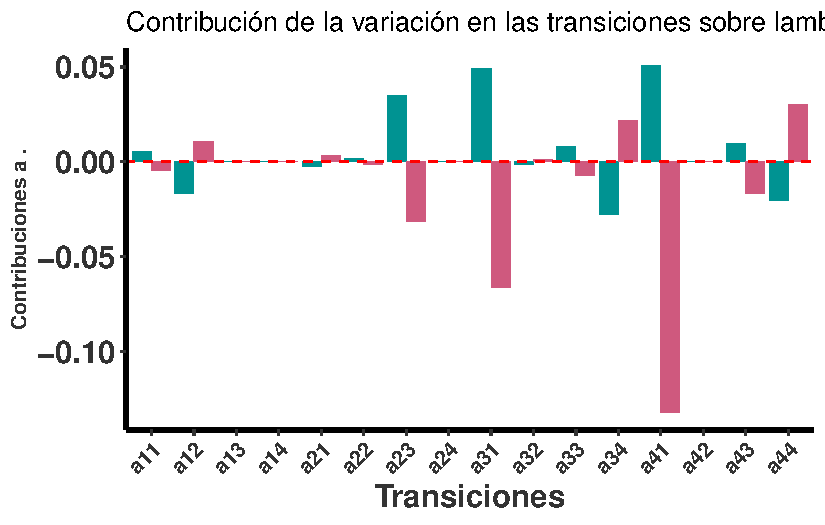
\includegraphics{114-LTRE_files/figure-pdf/LRE25-1.pdf}

\chapter{Alternativa de grafico (Adriana averigua cual de las opciones
de gráfico es
mejor)}\label{alternativa-de-grafico-adriana-averigua-cual-de-las-opciones-de-gruxe1fico-es-mejor}

\begin{Shaded}
\begin{Highlighting}[]
\FunctionTok{ggplot}\NormalTok{(pivot\_long, }\FunctionTok{aes}\NormalTok{(}\AttributeTok{x =}\NormalTok{ Transitions2, }\AttributeTok{y =}\NormalTok{ Contribution, }\AttributeTok{fill =}\NormalTok{ Species)) }\SpecialCharTok{+}
  \FunctionTok{geom\_bar}\NormalTok{(}\AttributeTok{stat =} \StringTok{"identity"}\NormalTok{, }\AttributeTok{position =} \StringTok{"dodge"}\NormalTok{) }\SpecialCharTok{+}
  \FunctionTok{labs}\NormalTok{(}
    \AttributeTok{title =} \StringTok{"Contribución de la variación en las transiciones sobre lambda"}\NormalTok{,}
    \AttributeTok{x =} \StringTok{"Transiciones"}\NormalTok{,}
    \AttributeTok{y =} \StringTok{"Contribuciones a λ"}
\NormalTok{  ) }\SpecialCharTok{+}
 \FunctionTok{rlt\_style\_fill}\NormalTok{()}\SpecialCharTok{+}
  \FunctionTok{facet\_wrap}\NormalTok{(}\SpecialCharTok{\textasciitilde{}}\NormalTok{Species) }\SpecialCharTok{+}
  \FunctionTok{theme}\NormalTok{(}\AttributeTok{axis.text.x =} \FunctionTok{element\_text}\NormalTok{(}\AttributeTok{angle =} \DecValTok{45}\NormalTok{, }\AttributeTok{hjust =} \DecValTok{1}\NormalTok{)) }\SpecialCharTok{+}
  \FunctionTok{geom\_hline}\NormalTok{(}\AttributeTok{yintercept =} \DecValTok{0}\NormalTok{, }\AttributeTok{linetype =} \StringTok{"dashed"}\NormalTok{, }\AttributeTok{color =} \StringTok{"red"}\NormalTok{) }\SpecialCharTok{+}
  \FunctionTok{theme}\NormalTok{(}\AttributeTok{legend.position =} \StringTok{"none"}\NormalTok{)}
\end{Highlighting}
\end{Shaded}

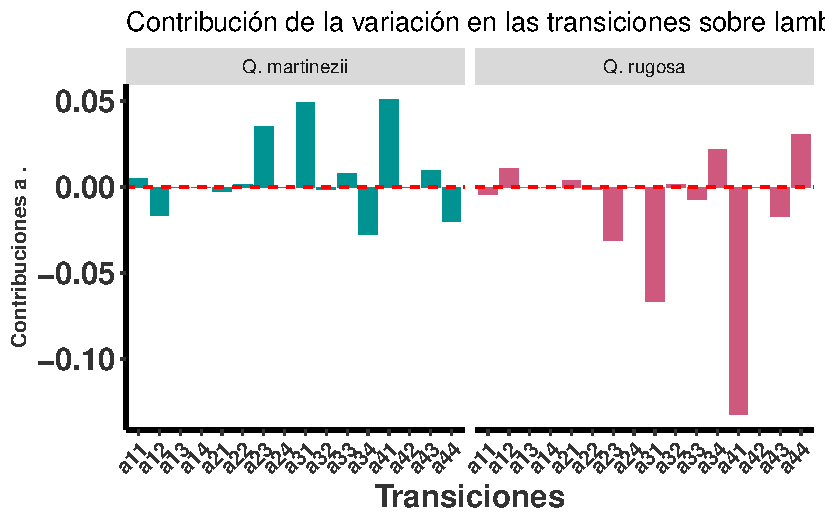
\includegraphics{114-LTRE_files/figure-pdf/LRE26-1.pdf}

Aquí se observa el efecto de las transiciones de las tasas vitales sobre
la variación en \emph{λ} para las dos especies de hospedero. Las barras
positivas indican contribuciones positivas a la variación en
\(\lambda\), mientras que las barras negativas indican contribuciones
negativas sobre \(\lambda\). El efecto de las transiciones de las tasas
vitales sobre la variación en \emph{λ} es diferente para cada especie de
hospedero, no solamente el efecto sobre las tasa vitales son diferentes
pero entre hospedero pero los cambios relativos. Lo que indica que las
dinámicas poblacionales de \emph{Oncidium brachyandrum} son
influenciadas por el hospedero en el que crece. Este patrón de cambios
de tasa vitales y su importancia relativa en la variación de \emph{λ}
necesita ser estudiado en más especies de orquídeas epífitas para
entender si es un patrón generalizado o no. Por consecuencia el proximo
paso es evaluar cual son la características de las especies de hospedero
que influyen en la dinámica poblacional de las orquídeas epífitas.

Enlace sobre ERTV https://bookdown.org/cdorm/lefko3gentle/ltre.html

Revisión:

RLT: 2025-06-11

\phantomsection\label{refs}
\begin{CSLReferences}{1}{0}
\bibitem[\citeproctext]{ref-birch1953experimental}
Birch L. 1953. Experimental background to the study of the distribution
and abundance of insects: I. The influence of temperature, moisture and
food on the innate capacity for increase of three grain beetles.
\emph{Ecology} 34:698--711.

\bibitem[\citeproctext]{ref-caswell1989analysis}
Caswell H. 1989b. Analysis of life table response experiments i.
Decomposition of effects on population growth rate. \emph{Ecological
Modelling} 46:221--237.

\bibitem[\citeproctext]{ref-caswell2000matrix}
Caswell H. 1989a. \emph{Matrix {P}opulation {M}odels}. Sinauer
Sunderland, MA.

\bibitem[\citeproctext]{ref-caswell2010life}
Caswell H. 2010. Life table response experiment analysis of the
stochastic growth rate. \emph{Journal of Ecology} 98:324--333.

\bibitem[\citeproctext]{ref-davison2010demographic}
Davison R, Jacquemyn H, Adriaens D, Honnay O, De Kroon H, Tuljapurkar S.
2010. Demographic effects of extreme weather events on a short-lived
calcareous grassland species: Stochastic life table response
experiments. \emph{Journal of Ecology} 98:255--267.

\bibitem[\citeproctext]{ref-gaoue2010effects}
Gaoue OG, Ticktin T. 2010. Effects of harvest of nontimber forest
products and ecological differences between sites on the demography of
african mahogany. \emph{Conservation Biology} 24:605--614.

\bibitem[\citeproctext]{ref-garcia2002reproductive}
Garcı́a MB, Ehrlén J. 2002. Reproductive effort and herbivory timing in a
perennial herb: Fitness components at the individual and population
levels. \emph{American Journal of Botany} 89:1295--1302.

\bibitem[\citeproctext]{ref-hansen1999multiannual}
Hansen TF, Stenseth NC, Henttonen H. 1999. Multiannual vole cycles and
population regulation during long winters: An analysis of seasonal
density dependence. \emph{The American Naturalist} 154:129--139.

\bibitem[\citeproctext]{ref-hart2021simulated}
Hart-Fredeluces G, Ticktin T, Lake FK. 2021. Simulated indigenous fire
stewardship increases the population growth rate of an understorey herb.
\emph{Journal of Ecology} 109:1133--1147.

\bibitem[\citeproctext]{ref-hastings2021effects}
Hastings A, Abbott KC, Cuddington K, Francis TB, Lai Y-C, Morozov A,
Petrovskii S, Zeeman ML. 2021. Effects of stochasticity on the length
and behaviour of ecological transients. \emph{Journal of the Royal
Society Interface} 18:20210257.

\bibitem[\citeproctext]{ref-hernandez2023exact}
Hernández CM, Ellner SP, Adler PB, Hooker G, Snyder RE. 2023. An exact
version of life table response experiment analysis, and the r package
exactLTRE. \emph{Methods in Ecology and Evolution} 14:939--951.

\bibitem[\citeproctext]{ref-hernandez2024natural}
Hernández CM, Ellner SP, Snyder RE, Hooker G. 2024. The natural history
of luck: A synthesis study of structured population models.
\emph{Ecology Letters} 27:e14390.

\bibitem[\citeproctext]{ref-horvitz1997relative}
Horvitz C, Schemske DW, Caswell H. 1997. The relative {``importance''}
of life-history stages to population growth: Prospective and
retrospective analyses. In: \emph{Structured-population models in
marine, terrestrial, and freshwater systems}. Springer, 247--271.

\bibitem[\citeproctext]{ref-jacquemyn2012stochastic}
Jacquemyn H, Brys R, Davison R, Tuljapurkar S, Jongejans E. 2012.
Stochastic LTRE analysis of the effects of herbivory on the population
dynamics of a perennial grassland herb. \emph{Oikos} 121:211--218.

\bibitem[\citeproctext]{ref-levin1996demographic}
Levin L, Caswell H, Bridges T, DiBacco C, Cabrera D, Plaia G. 1996.
Demographic responses of estuarine polychaetes to pollutants: Life table
response experiments. \emph{Ecological Applications} 6:1295--1313.

\bibitem[\citeproctext]{ref-miriti2001effects}
Miriti MN, Joseph Wright S, Howe HF. 2001. The effects of neighbors on
the demography of a dominant desert shrub (\emph{{A}mbrosia {d}umosa}).
\emph{Ecological Monographs} 71:491--509.

\bibitem[\citeproctext]{ref-mondragon2009population}
Mondragón D. 2009. Population viability analysis for \emph{{G}uarianthe
{a}urantiaca}, an ornamental epiphytic orchid harvested in {S}outheast
{M}{é}xico. \emph{Plant Species Biology} 24:35--41.

\bibitem[\citeproctext]{ref-nordbakken2004demography}
Nordbakken J-F, Rydgren K, Økland R. 2004. Demography and population
dynamics of \emph{{D}rosera {a}nglica} and \emph{{D}. {r}otundifolia}.
\emph{Journal of Ecology} 92:110--121.

\bibitem[\citeproctext]{ref-oli2001effect}
Oli MK, Slade NA, Dobson FS. 2001. Effect of density reduction on uinta
ground squirrels: Analysis of life table response experiments.
\emph{Ecology} 82:1921--1929.

\bibitem[\citeproctext]{ref-ramirez2021host}
Ramı́rez Martı́nez A. 2021. Host tree effect on demography and phenology
of epiphytic species. PhD thesis Thesis. Instituto Polit{é}cnico
Nacional. Centro Interdisciplinario de Investigaci{ó}n.

\bibitem[\citeproctext]{ref-schmidt2011matrix}
Schmidt IB, Mandle L, Ticktin T, Gaoue OG. 2011. What do matrix
population models reveal about the sustainability of non-timber forest
product harvest? \emph{Journal of Applied Ecology} 48:815--826.

\bibitem[\citeproctext]{ref-stott2012beyond}
Stott I, Hodgson DJ, Townley S. 2012. Beyond sensitivity: Nonlinear
perturbation analysis of transient dynamics. \emph{Methods in Ecology
and Evolution} 3:673--684.

\bibitem[\citeproctext]{ref-stott2011framework}
Stott I, Townley S, Hodgson DJ. 2011. A framework for studying transient
dynamics of population projection matrix models. \emph{Ecology Letters}
14:959--970.

\bibitem[\citeproctext]{ref-sun2019multivariate}
Sun W, Yuan X, Liu Z-J, Lan S, Tsai W, Zou S-Q. 2019. Multivariate
analysis reveals phenotypic diversity of \emph{{E}uscaphis {j}aponica}
population. \emph{PloS one} 14:e0219046.

\bibitem[\citeproctext]{ref-teitel2016assessing}
Teitel Z, Klimowski A, Campbell LG. 2016. Assessing the effects of
hybridization and precipitation on invasive weed demography using
strength of selection on vital rates. \emph{BMC Evolutionary Biology}
16:1--13.

\bibitem[\citeproctext]{ref-timsina2021six}
Timsina B, Kindlmann P, Münzbergová Z, Rokaya MB. 2021. Six-year
demographic study of the terrestrial orchid, \emph{{C}repidium
{a}cuminatum}: Implications for conservation. \emph{Frontiers in Ecology
and Evolution} 9:676993.

\end{CSLReferences}


\backmatter


\end{document}
